\documentclass[11pt,a4paper,oneside]{report}             % Single-side
%\documentclass[11pt,a4paper,twoside,openright]{report}  % Duplex

%\PassOptionsToPackage{chapternumber=Huordinal}{magyar.ldf}
\usepackage{t1enc}
\usepackage[latin2]{inputenc}
\usepackage{amsmath}
\usepackage{amssymb}
\usepackage{enumerate}
\usepackage[thmmarks]{ntheorem}
\usepackage{graphics}
\usepackage{epsfig}
\usepackage{listings}
\usepackage{color}
%\usepackage{fancyhdr}
\usepackage{lastpage}
\usepackage{anysize}
\usepackage[magyar]{babel}
\usepackage{sectsty}
\usepackage{setspace}  % Ettol a tablazatok, abrak, labjegyzetek maradnak 1-es sorkozzel!
\usepackage[hang]{caption}
\usepackage{hyperref}
\usepackage{float}
\usepackage{breakurl} 

%--------------------------------------------------------------------------------------
% Main variables
%--------------------------------------------------------------------------------------
\newcommand{\vikszerzo}{B�jti Paszk�l}
\newcommand{\vikkonzulens}{V�r�s Andr�s, Dr. Bartha Tam�s}
\newcommand{\vikcim}{Megb�zhat� kommunik�ci�s kapcsolattal rendelkez� f�ldi ir�ny�t� �llom�s fejleszt�se UAV-hoz}
\newcommand{\viktanszek}{M�r�stechnika �s Inform�ci�s Rendszerek Tansz�k}
\newcommand{\vikdoktipus}{Szakdolgozat}

%--------------------------------------------------------------------------------------
% Page layout setup
%--------------------------------------------------------------------------------------
% we need to redefine the pagestyle plain
% another possibility is to use the body of this command without \fancypagestyle
% and use \pagestyle{fancy} but in that case the special pages
% (like the ToC, the References, and the Chapter pages)remain in plane style

\pagestyle{plain}
%\setlength{\parindent}{0pt} % �ttekinthet�bb, angol nyelv� dokumentumokban jellemz�
%\setlength{\parskip}{8pt plus 3pt minus 3pt} % �ttekinthet�bb, angol nyelv� dokumentumokban jellemz�
\setlength{\parindent}{12pt} % magyar nyelv� dokumentumokban jellemz�
\setlength{\parskip}{0pt}    % magyar nyelv� dokumentumokban jellemz�

\marginsize{35mm}{25mm}{15mm}{15mm} % anysize package
\setcounter{secnumdepth}{0}
\sectionfont{\large\upshape\bfseries}
\setcounter{secnumdepth}{2}
\singlespacing
\frenchspacing

%--------------------------------------------------------------------------------------
%	Setup hyperref package
%--------------------------------------------------------------------------------------
\hypersetup{
    bookmarks=true,            % show bookmarks bar?
    unicode=false,             % non-Latin characters in Acrobat�s bookmarks
    pdftitle={\vikcim},        % title
    pdfauthor={\vikszerzo},    % author
    pdfsubject={\vikdoktipus}, % subject of the document
    pdfcreator={\vikszerzo},   % creator of the document
    pdfproducer={Producer},    % producer of the document
    pdfkeywords={keywords},    % list of keywords
    pdfnewwindow=true,         % links in new window
    colorlinks=true,           % false: boxed links; true: colored links
    linkcolor=black,           % color of internal links
    citecolor=black,           % color of links to bibliography
    filecolor=black,           % color of file links
    urlcolor=black             % color of external links
}

%--------------------------------------------------------------------------------------
% Set up listings
%--------------------------------------------------------------------------------------
\lstset{
	basicstyle=\scriptsize\ttfamily, % print whole listing small
	keywordstyle=\color{black}\bfseries\underbar, % underlined bold black keywords
	identifierstyle=, 					% nothing happens
	commentstyle=\color{white}, % white comments
	stringstyle=\scriptsize\sffamily, 			% typewriter type for strings
	showstringspaces=false,     % no special string spaces
	aboveskip=3pt,
	belowskip=3pt,
	columns=fixed,
	backgroundcolor=\color{lightgray},
} 		
\def\lstlistingname{lista}	

%--------------------------------------------------------------------------------------
%	Some new commands and declarations
%--------------------------------------------------------------------------------------
\newcommand{\code}[1]{{\upshape\ttfamily\scriptsize\indent #1}}

% define references
\newcommand{\figref}[1]{\ref{fig:#1}.}
\renewcommand{\eqref}[1]{(\ref{eq:#1})}
\newcommand{\listref}[1]{\ref{listing:#1}.}
\newcommand{\sectref}[1]{\ref{sect:#1}}
\newcommand{\tabref}[1]{\ref{tab:#1}.}

\DeclareMathOperator*{\argmax}{arg\,max}
%\DeclareMathOperator*[1]{\floor}{arg\,max}
\DeclareMathOperator{\sign}{sgn}
\DeclareMathOperator{\rot}{rot}
\definecolor{lightgray}{rgb}{0.95,0.95,0.95}

\usepackage[T1]{fontenc}
\usepackage[scaled]{beramono}

\definecolor{bluekeywords}{rgb}{0.13,0.13,1}
\definecolor{greencomments}{rgb}{0,0.5,0}
\definecolor{redstrings}{rgb}{0.9,0,0}

\usepackage{listings}
\lstset{
language=[Sharp]C,
basicstyle=\small,
showspaces=false,
showtabs=false,
breaklines=true,
showstringspaces=false,
breakatwhitespace=true,
escapeinside={(*@}{@*)},
commentstyle=\color{greencomments},
keywordstyle=\color{bluekeywords}\bfseries,
stringstyle=\color{redstrings},
basicstyle=\ttfamily
}

\author{\vikszerzo}
\title{\viktitle}
\includeonly{
%
	titlepage,%
	declaration,%
	abstract,%
	%introduction,%
	%chapter0, %
	elozmenyek,%
	tervezes,%
	kivitelezes,%
	%ertekeles,%
	chapter4,%
	appendices,%
}
%--------------------------------------------------------------------------------------
%	Setup captions
%--------------------------------------------------------------------------------------
\captionsetup[figure]{
%labelsep=none,
%font={footnotesize,it},
%justification=justified,
width=.75\textwidth,
aboveskip=10pt}

\renewcommand{\captionlabelfont}{\small\bf}
\renewcommand{\captionfont}{\footnotesize\it}

%--------------------------------------------------------------------------------------
% Table of contents and the main text
%--------------------------------------------------------------------------------------
\begin{document}
\singlespacing



\pagenumbering{arabic}
\onehalfspacing
%--------------------------------------------------------------------------------------
%	The title page
%--------------------------------------------------------------------------------------
\begin{titlepage}
\begin{center}

\includegraphics[width=60mm,keepaspectratio]{figures/BMElogo.png}\\
\vspace{0.3cm}
\textbf{Budapesti M�szaki �s Gazdas�gtudom�nyi Egyetem}\\
\textmd{Villamosm�rn�ki �s Informatikai Kar}\\
\textmd{\viktanszek}\\[5cm]

\vspace{0.4cm}
{\huge \bfseries \vikcim}\\[0.8cm]
\vspace{0.5cm}
\textsc{\Large \vikdoktipus}\\[1cm]


\textsc{\emph{K�sz�tette}}\\
\textsc{\vikszerzo}\\[7cm]

\textsc{\emph{Konzulensek}}\\
\textsc{\vikkonzulens}\\

%\begin{tabular}{cc}
% \makebox[7cm]{\emph{K�sz�tette}} & \makebox[7cm]{\emph{Konzulensek}} \\
% \makebox[7cm]{\vikszerzo} & \makebox[7cm]{\vikkonzulens}
%\end{tabular}

\vfill
{\large \today}
\end{center}
\end{titlepage}



\tableofcontents\vfill
%--------------------------------------------------------------------------------------
% Nyilatkozat
%--------------------------------------------------------------------------------------
\begin{center}
\large
\textbf{HALLGAT�I NYILATKOZAT}\\
\end{center}

Alul�rott \emph{\vikszerzo}, szigorl� hallgat� kijelentem, hogy ezt a szakdolgozatot meg nem engedett seg�ts�g n�lk�l, saj�t magam k�sz�tettem, csak a megadott forr�sokat (szakirodalom, eszk�z�k stb.) haszn�ltam fel. Minden olyan r�szt, melyet sz� szerint, vagy azonos �rtelemben, de �tfogalmazva m�s forr�sb�l �tvettem, egy�rtelm�en, a forr�s megad�s�val megjel�ltem.

Hozz�j�rulok, hogy a jelen munk�m alapadatait (\vikszerzo, \vikcim, angol �s magyar nyelv� tartalmi kivonat, 2013, \vikkonzulens) a BME VIK nyilv�nosan hozz�f�rhet� elektronikus form�ban, a munka teljes sz�veg�t pedig az egyetem bels� h�l�zat�n kereszt�l (vagy autentik�lt felhaszn�l�k sz�m�ra) k�zz�tegye. Kijelentem, hogy a beny�jtott munka �s annak elektronikus verzi�ja megegyezik. D�k�ni enged�llyel titkos�tott diplomatervek eset�n a dolgozat sz�vege csak 3 �v eltelte ut�n v�lik hozz�f�rhet�v�.

\begin{flushleft}
\vspace*{1cm}
Budapest, \today
\end{flushleft}

\begin{flushright}
 \vspace*{1cm}
 \makebox[7cm]{\rule{6cm}{.4pt}}\\
 \makebox[7cm]{\emph{\vikszerzo}}\\
 \makebox[7cm]{hallgat�}
\end{flushright}
\thispagestyle{empty}

\vfill
\clearpage
\thispagestyle{empty} % an empty page


%----------------------------------------------------------------------------
% Abstract in hungarian
%----------------------------------------------------------------------------
\chapter*{Kivonat}\addcontentsline{toc}{chapter}{Kivonat}

Napjainkban egyre nagyobb teret h�d�t a pil�ta n�lk�li l�gi j�rm�vek alkalmaz�sa.
Az 1960-as �vekben a hadsz�nt�ren jelentek meg el�sz�r, ahol megfigyel�sre, felder�t�sre �s olyan feladatokra haszn�lt�k, ahol kock�zatos lett volna emberi �letet vesz�lyeztetni.
Az ut�bbi �vekben praktikuss�ga, alacsony �zemeltet�si k�lts�gei miatt m�s ter�leteken is hasznosnak bizonyult ez a technol�gia, pl. geol�gia mint�zatok kutat�sa, mely az emberi perspekt�v�b�l nehezen �szlelhet�, t�zolt�s�gi alakulatok koordin�l�sa, otthoni hobby felhaszn�l�s. 

Az MTA-SZTAKI Rendszer �s Ir�ny�t�selm�leti Kutat�laborat�rium�ban kidolgozott szab�lyoz� algoritmusok gyakorlatba val� �t�ltet�s�re egy pil�ta n�lk�li j�rm�vet hoztak l�tre, mely a biztons�gos �zemeltet�s mellett, illetve az esetlegesen el�fordulhat� hib�k ellen redund�ns hardware elemekkel v�dekezik. Szakdolgozatom keret�ben ennek a rep�l�nek a f�ldi �llom�s�t dolgoztam ki, mely a redund�nsan k�ld�tt r�di�jelek feldolgoz�s�ra �s megfelel� megjelen�t�sre haszn�land�. A f�ldi szem�lyzet mozg� t�rk�p alap� vizualiz�ci�n l�thatja az akt�v �tvonalpontokat �s a g�p �tvonal�t, a diagnosztikai adatokat �s esetleges hib�kat egy m�sik n�zetben �ttekintheti. Lehet�s�g ny�lik rep�l�si terv meghat�roz�s�ra �s felt�lt�s�re a rep�l�re, melynek fordul�pontjait k�veti.

%----------------------------------------------------------------------------
% Abstract in english
%----------------------------------------------------------------------------
\chapter*{Abstract}\addcontentsline{toc}{chapter}{Abstract}
Nowadays the use of unmanned aircrafts shows an increasing number.
UAVs appeared for the first time in the 1960s in military use, where it would have been risky to endanger human life, for example observation and discovery tasks.

In recent years, because of it's low running costs and practical usage, this technology has proved that it is useful in other areas , eg.  geology research, helping fire units and hobby use.

MTA-SZTAKI Rendszer �s Ir�ny�t�selm�leti Kutat�laborat�rium has developed control algorithms, which was elaborated into practice by an unmanned vehicle. In addition to the safe operation and for potentially active faults occur, it is defended with redundant hardware elements. In the context of this thesis  I worked out a software for the ground station of this airplane, which is used to process and display the redundantly sent radio signals. The ground staff can see a map-based visualization of the active waypoints and routes the machine, diagnostic data. It is possible to create and upload flight plan, which contains the turning points which the aircraft needs to follow.

\vfill


%%----------------------------------------------------------------------------
\chapter*{Bevezet�}\addcontentsline{toc}{chapter}{Bevezet�}
%----------------------------------------------------------------------------


\cite{bib:uav}A pil�ta n�lk�li l�gi j�rm� gondolata eg�szen a XX. sz�zad elej�re ny�lik vissza, mikor az I. vil�gh�bor�ban egy olyan t�vir�ny�t�s� rep�l�t alkottak, mely robban�szerrel a fed�lzeten a c�lpontba csap�dva okozott k�rt.
K�s�bb a vietn�mi h�bor�ban t�bb mint 3000 k�ldet�sben vett r�szt ilyen rep�l� �s mind�ssze 554 veszett oda. A technol�giai korl�tok miatt a f� funkcionalit�sa vide� felv�tel k�sz�t�se egy meghat�rozott �tvonalon (�ltal�ban egyenes vonal, k�r�kkel kieg�sz�tve) rep�lve, majd a b�zisra val� vissza�rkez�s. 
A r�di�technika fejl�d�se miatt egyre �sszetettebb feladatok elv�gz�s�re lettek k�pesek. A nagyobb �tviteli sebess�gnek k�sz�nhet�en val�s id�ben, monitoron kereszt�l kezelheti az oper�tor a t�vir�ny�t�s� rep�l�t. A mai UAV-k t�bb �zemm�dot is t�mogatnak, egyik az el�bb eml�tett t�vir�ny�t�s, m�sik a fed�lzeti intelligenci�ra hagyatkoz�. Mind a hagyom�nyos rep�l�iparban, mind ebben az �r�ban, sz�ks�ges �s c�lszer� az emberi terhel�s cs�kkent�se, utassz�ll�t� g�pek eset�ben is a robotpil�ta elv�gez minden olyan korrekci�t, melyet azel�tt a pil�ta folyamatos figyel�s�vel, koncentr�ci�j�val lehetett el�rni. A modern integr�ci�nak k�sz�nhet�en, olyan fejlett feldolgoz�egys�ggel dolgozhatjuk fel az adatokat, melyeknek nem jelent�s a fogyaszt�sa, nem foglalnak sok helyet. A szenzorokb�l �rkez� inform�ci�kra, az algoritmusoknak k�sz�nhet�en �gy k�pes reag�lni, hogy az nem vesz�lyezteti a rep�l� leveg�ben marad�s�t. �m hi�ba a fejlett hardware, a val�ban automatikus �zemeltet�s m�g mindig t�voli c�l, emberi beavatkoz�s mindig is kelleni fog olyan helyzetekben melyre nincs el�re felk�sz�tve az intelligenci�ja. Ilyen esetekben l�tfontoss�g�, hogy az oper�tor l�ssa a g�p aktu�lis poz�ci�j�t, diagnosztikai adatait. 

Feladatom egy olyan grafikus felhaszn�l�i fel�lettel ell�tott f�ldi ir�ny�t� �llom�s kifejleszt�se egy biztons�gkritikus robotrep�l�h�z, ami k�pes redund�ns kommunik�ci�s csatorn�n k�ld�tt adatok kezel�s�re �s megjelen�t�s�re. Ehhez sz�ks�ges megoldanom a kapcsolatot biztos�t� modem jeleinek v�tel�t. Mivel hibat�r� kialak�t�sa r�v�n redund�nsan szerelt, �gy a p�rhuzamos csatorn�kon �rkez� adatok egym�st�l val� elt�r�s�nek a kijelz�se is megval�s�tand�. Az elt�r�snek t�bb oka is lehets�ges, el�fordulhat, hogy az egyik meghib�sod�s�b�l k�vetkez�en nem k�ld semmilyen �rt�ket vagy amit k�ld az teljesen hib�s, 
Tov�bb�, ez a program a f�ld�n tart�zkod� szem�lyzet kiszolg�l�s�ra k�sz�l, �gy ami a legfontosabb, hogy �k a rep�l�vel kapcsolatos inform�ci�kat k�nnyen �rtelmezhess�k. �gy sz�ks�ges megoldani, hogy a kialak�tand� fel�let felhaszn�l�bar�t legyen, ehhez t�bb n�zeti oldal sz�ks�ges: 
\begin{itemize}
\item Egy �ttekint� k�perny�, mely a legfontosabb adatokat jelen�ti meg a rep�l�vel kapcsolatban ( poz�ci�, sebess�g, ir�ny)
\item Egy tervez� modul, amin a lerep�lend� �tvonalhoz tartoz� fordul�pontok kijel�l�se lehets�ges
\item Egy diagnosztikai n�zet, melyen az alacsonyabb priorit�s� adatok tekinthet�ek �t
\end{itemize}
%\chapter{A feladatki�r�s pontos�t�sa �s r�szletes elemz�se}

\chapter{El�zm�nyek}


\section{Motiv�ci�}
 
Az MTA SZTAKI Rendszer �s Ir�ny�t�selm�leti Kutat�laborat�rium�ban foly� kutat�sok eredm�ny�nek demonstr�l�s�ra sz�ks�g volt egy k�zzelfoghat� eszk�z megalkot�s�ra. A kifejlesztett szab�lyoz� algoritmusok m�k�d�s�nek bemutat�s�nak az egyik legl�tv�nyosabb m�dja egy rep�l�g�p ir�ny�t�sa. Egy stabil rep�l�si tulajdons�gokkal b�r� rep�l� leveg�ben tart�sa sem trivi�lis, sz�ks�g van a korm�nyszervek harmonikus mozgat�s�ra, a tol�er� szab�lyz�s�ra. Ezen t�lmen�en ha feladatokkal l�tjuk el, pl. fordul�pontokat k�vetve felt�rk�pezni az alatta l�v� ter�letet, m�r sz�molni kell a sz�llel, mely elt�r�theti az �tvonal�r�l, felsz�ll� l�g�ramlatokkal, melyek ellen gyors reag�l�ssal kell v�laszolnia. Mivel egy teljesen felszerelt rep�l� �ssze�ll�t�sa, felprogramoz�sa nagy szak�rtelmet, sok id�t, energi�t ig�nyel �s nem utols� sorban anyagi r�ford�t�st, egy esetleges meghib�sod�s jelent�s k�rt okozna. Ezen okok miatt felmer�lt az ig�ny a rep�l� megb�zhat�s�g�nak n�vel�s�re, �gy a most folyamatban l�v� ``Nagy megb�zhat�s�g� pil�ta n�lk�li l�gij�rm� projekt'' keret�ben egy olyan avionikai rendszer fejleszt�se is folyik, amelyben c�l minden egyes rep�l�g�p alrendszer meghib�sod�s�nak diagnosztiz�l�sa, a diagnosztikai inform�ci�kat felhaszn�lva a rep�l�g�p �tkonfigur�l�sa. 


\section{Rep�l�g�p fel�p�t�se}

A jelenlegi rep�l� egy saj�t �p�t�s� 3.2 m feszt�vols�g� modell, melybe diagnosztikai �s hibadetekci�s c�lokra egyedi tervez�s� komponensek ker�ltek. A kommerci�lis c�lokra sz�nt szerv� motorok nem szolg�lnak el�g inform�ci�val a kit�r�s�kr�l, fogyaszt�sukr�l, ez�rt ezek m�r�s�r�l gondoskodni kellett.

\begin{figure}[H]
	\centering
	\resizebox{12cm}{!}{
		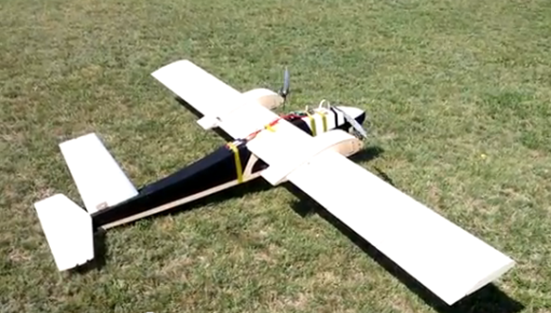
\includegraphics{figures/orca.png}}
	\caption{}
	\label{fig:sys}
\end{figure}


\subsection{Architekt�ra}

Els�dleges szempont, hogy egy komponens meghib�sod�sa ne okozza a g�p veszt�t, teh�t a rendszerben ne maradjon SPOF \footnote{Single Point Of Failure, olyan meghib�sod�s, mely ha bek�vetkezik, az eg�sz rendszer le�ll�s�hoz vezet}. Ezt redundanci�val �rhetj�k el, mely sor�n a rep�l�g�pen duplik�ljuk azokat az elemeket, melyek n�lk�l�zhetetlenek a leveg�ben marad�s�hoz:
\begin{itemize}
\item motor
\item korm�nyfel�letek �s ezeket mozgat� motorok
\item t�pell�t�s
\item k�zponti sz�m�t�g�p
\end{itemize}

A rep�l� m�ret�b�l ad�d�an t�rbeli szepar�ci�val nem lehets�ges a megb�zhat�s�g n�vel�se, mint pl. harci rep�l�g�pek fed�lzeti sz�m�t�g�pein�l, melyek a tal�lat kock�zata miatt elsz�rva, ak�r 4--5x-ve vannak.

\begin{figure}[H]
	\centering
	\resizebox{13cm}{!}{
		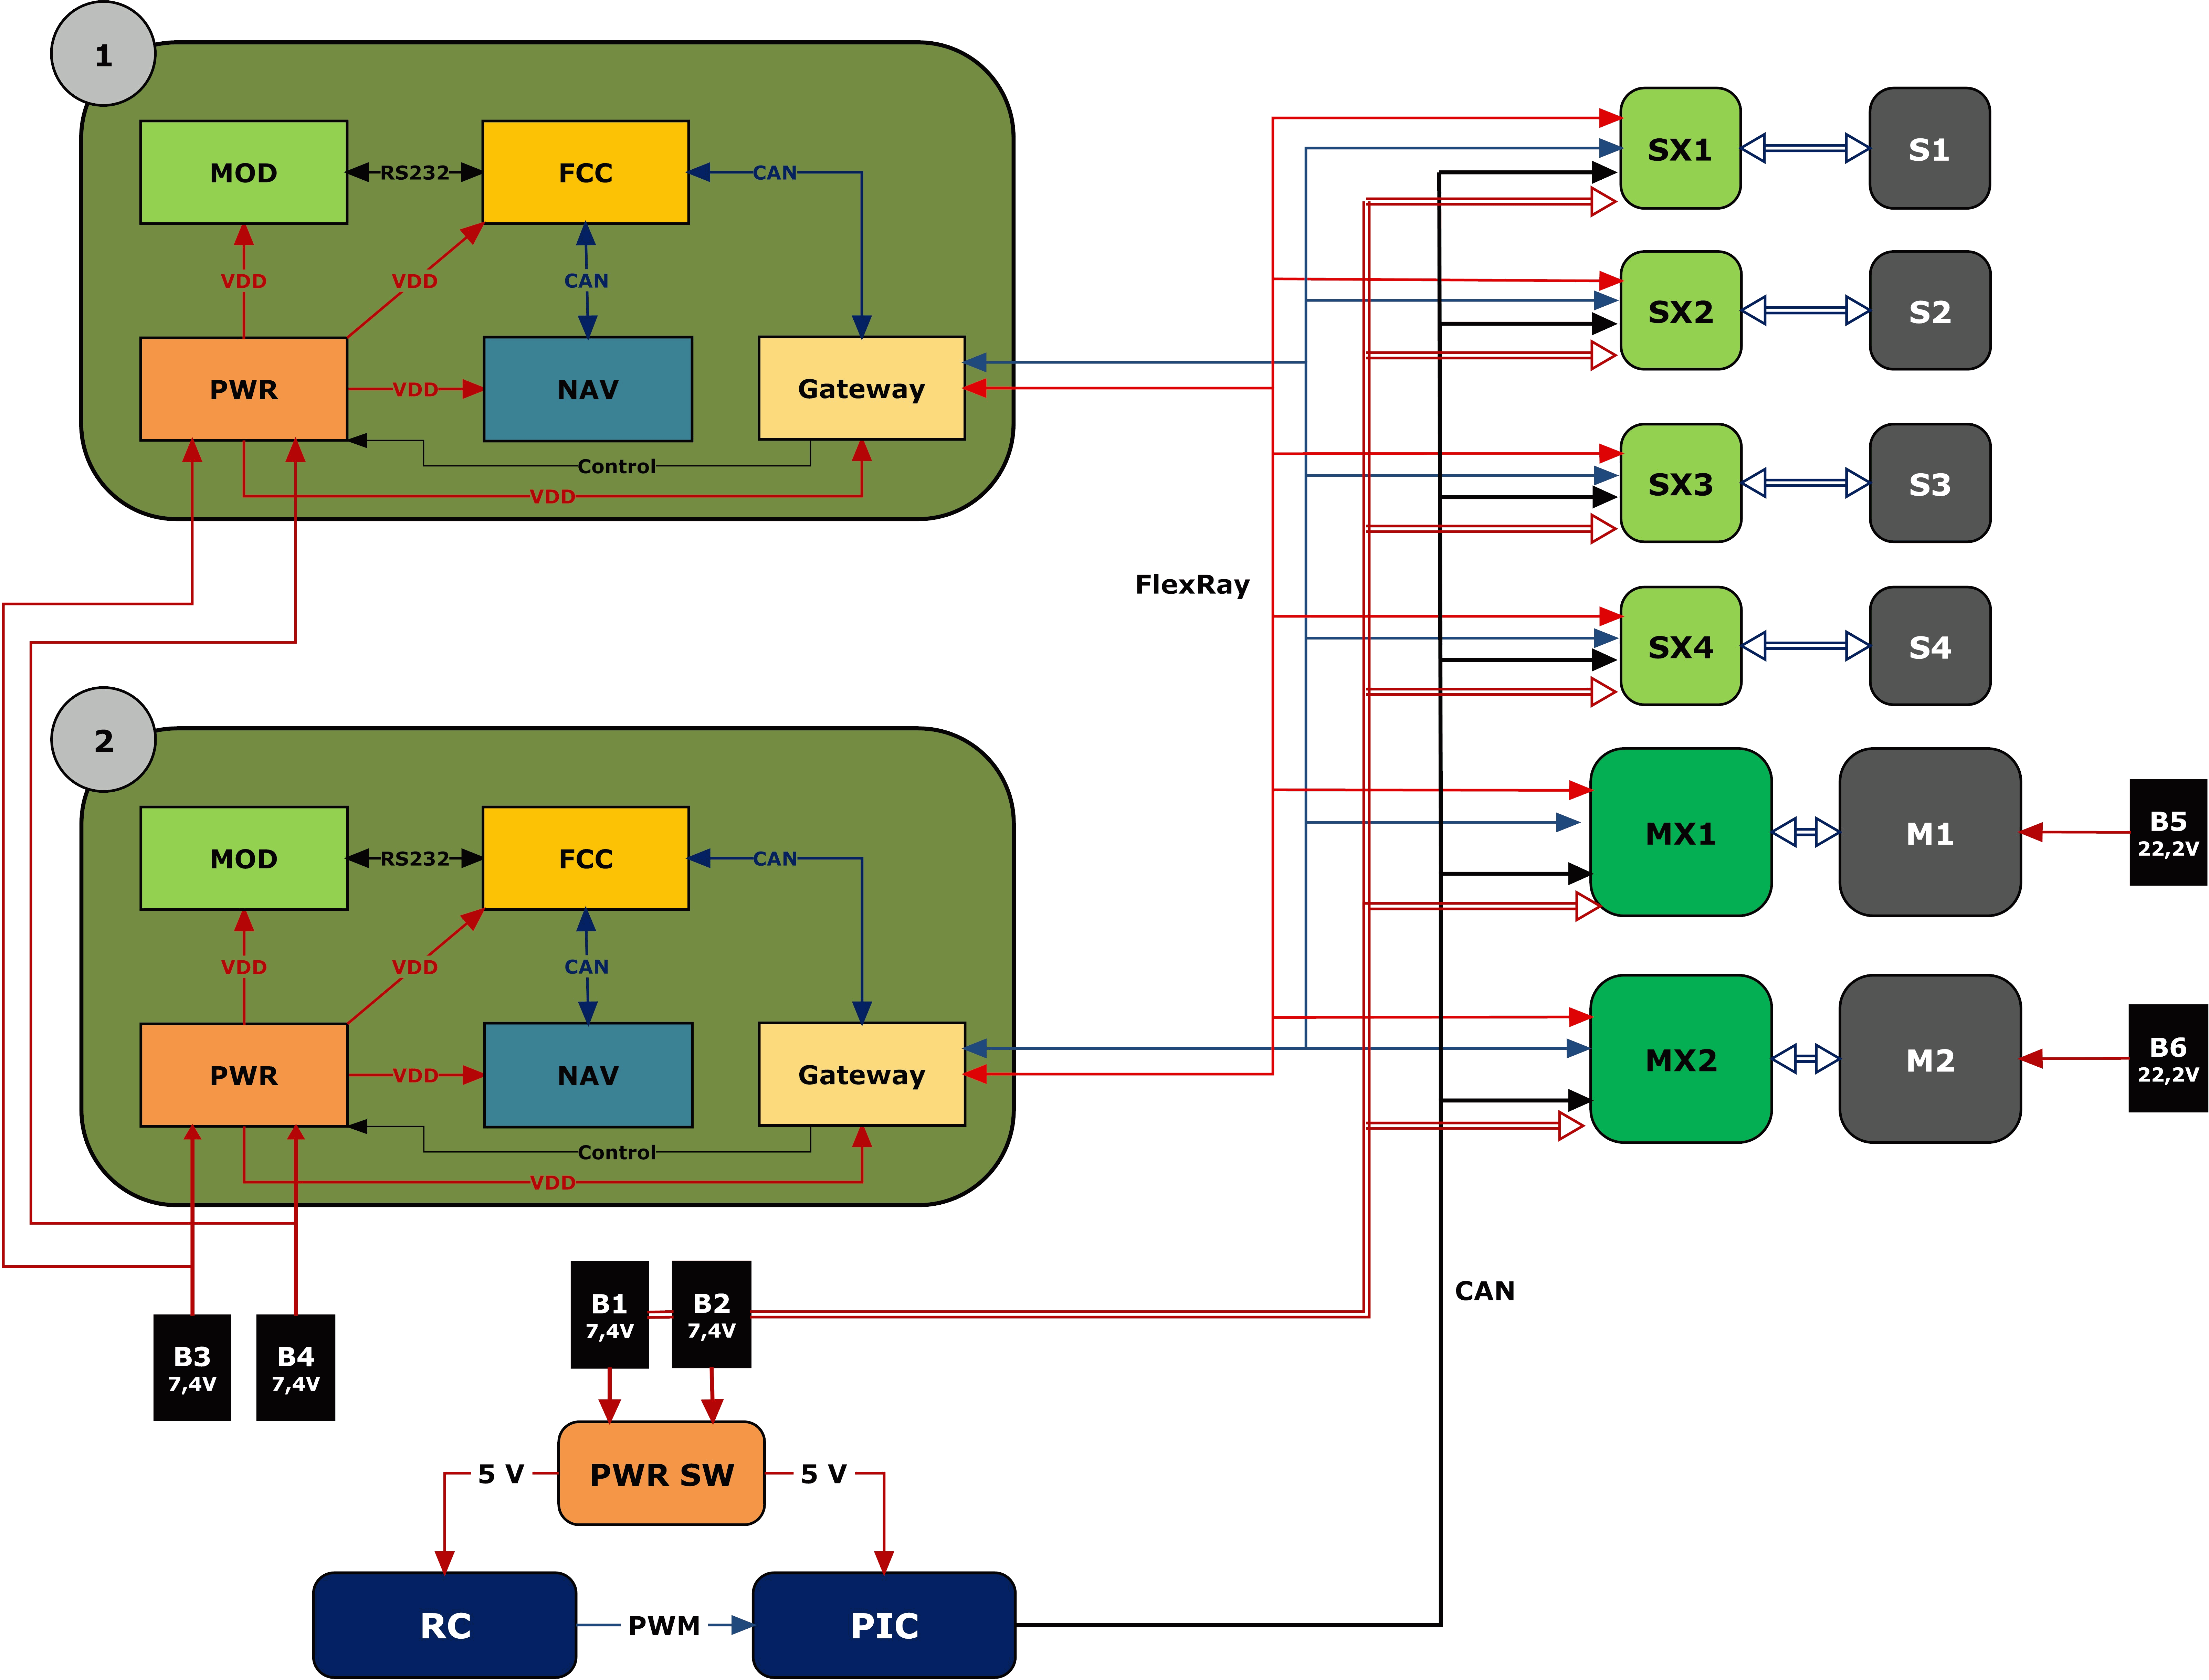
\includegraphics{figures/sys.png}}
	\caption{}
	\label{fig:sys}
\end{figure}

\figref{sys} �br�n l�that� a kialak�tott architekt�ra. Elemei:

\begin{itemize}
\item \textbf{FCC} Flight Controll Computer, rep�l�g�p ir�ny�t�sa
\item \textbf{NAV} GPS, nyom�sm�r�, orient�ci�m�r�
\item \textbf{MOD} modem, kommunik�ci�
\item \textbf{Gateway} CAN-FlexRay �tj�r�st biztos�t
\item \textbf{PWR} fesz�lts�gv�laszt�
\item \textbf{M1, M2} motorok
\item \textbf{S1, S2, S3, S4} szerv�k
\item \textbf{Sx, Mx} szab�lyz�elektronika

\end{itemize}

A k�zponti sz�m�t�g�pek(�br�n z�lddel jel�lve 1-es 2-es) 1--1 szendvics panelen helyezkednek el, k�zponti elem�k az FCC, mely az ir�ny�t�s�rt felel�s. A navig�ci�s (NAV) eszk�z szolg�ltatja a GPS-b�l �rkez� magass�g �s poz�ci� adatokat, az IMU\footnote{}-b�l �rkez� orient�ci�t, a nyom�sm�r�b�l a l�gsebess�g �s magass�g �rt�keket. Ezen egy mikrokontroller el�feldolgoz�st v�gez, �gy m�r csak a t�nylegesen feldolgozand� inform�ci�val kell az FCC-nek sz�molnia. Az FCC �s a NAV k�z�tti kommunik�ci� CAN buszon kereszt�l zajlik. Az �br�n l�that� S �s M-mel jel�lt elemek rendre a szerv� motorok �s a meghajt�s�rt felel�s motorok, melyek redund�ns FlexRay kommunik�ci�s csatorn�n kapj�k az utas�t�sokat az FCC-b�l. A CAN--FlexRay �s FlexRay--CAN �talak�t�st a Gateway egys�g v�gzi. A szerv�k �s motorok nem szolg�lnak el�g inform�ci�val saj�t �llapotukr�l, �gy ezek �t vannak alak�tva, hogy a FlexRay h�l�zatra illeszt�s�rt felel�s szab�lyoz�elektronik�juk (Sx, Mx) megfelel�en m�k�dhessen. Ezekre b�rmilyen szab�lyz�algoritmus �rhat�, hibadiagnosztikai c�lokra fault detection filtert vagy K�rm�n sz�r� alkalmazhat�. A szerv�k m�gneses enk�dere a kit�r�sr�l, a motorok elektronik�ja a fogyaszt�sr�l ad inform�ci�t. 
A dolgozat szempontj�b�l a leg�rdekesebb egys�g a modem (MOD) mely az FCC-vel soros porton kommunik�l.
Hibat�r�sb�l ad�d�an az energiaforr�sok is redund�nsan szerepelnek, a k�zponti sz�m�t�g�pek a B3 �s B4-gyel jel�lt akkumul�torb�l nyerhetnek energi�t, a v�laszt�st a PWR n�ven jelzett egys�g v�gzi. K�l�nb�z� strat�gi�k v�laszthat�k az akkumul�tor �tkapcsol�s�t illet�en, lehets�ges mindig a legnagyobb fesz�lts�ggel oper�l�t v�lasztani vagy egyiket lemer�teni bizonyos sz�zal�kig �s ezut�n v�ltani. A B5 �s B6 a motorokat hivatottak kiszolg�lni, ezek a legnagyobb fogyaszt�s�ak, �gy ezek kapacit�sa a legnagyobb. B1 �s B2 biztos�tja az aktu�toroknak, az hozz�juk tartoz� vez�rl�knek az �ramforr�st.
Tov�bb�, mivel a rep�l�g�p jelenleg csak t�vir�ny�t�ssal tud felsz�llni, �gy a t�vvez�rl� egys�g (RC) �s a PWM-CAN �talak�t�s�rt felel�s PIC is ezt a 2 akkumul�tort haszn�lja. A PIC k�zvetlen�l az szab�lyz� elektronik�khoz csatlakozik CAN interface-en, ez a legk�zvetlenebb m�dja a k�zi ir�ny�t�snak.

\subsection{Kommunik�ci�}
A fed�lzeti MOD egys�g egy \cite{bib:xbee} XBee-PRO 868 t�pus� modem, mely alacsony fogyaszt�sa �s nagy hat�t�vols�ga miatt ide�lis egy ilyen k�rnyezetbe. Vev� oldalon ugyanilyen modem tal�lhat� duplik�ltan, mely szint�n soros porton k�ldi a f�ldi �llom�snak a vett jelet, a modemek k�z�tt l�v� vezet�k n�lk�li protokoll: 802.15.4, mellyel a \sectref{prot} fejezet foglalkozik.

\subsubsection{Vezet�k n�lk�li modem}

A kiv�lasztott modem k�tf�lek�ppen k�pes kommunik�lni:

\begin{itemize}
\item API csomagk�ld�s
\item AT transzparens
\end{itemize}

\textbf{API} m�dban egy eszk�z t�bb eszk�zt�l tud csomagokat venni, ha egy csomag meg�rkezik a k�ld�t�l a fogad�ig, egy ACK\footnote{Acknowledgement, nyugt�z� �zenet} �zenettel v�laszol, ha ezt nem kapja meg, a csomagot �jrak�ldi, lehet�s�g van broadcast �zenetek k�ld�s�re is, melyet minden eszk�z megkap. Egy csomag t�bbek k�zt tartalmazza a k�ld� �s a fogad� c�m�t, az adatot �s adatintegrit�s c�lj�b�l checksum mez�j�ben �sszes�tve csomag tartalm�t.


\textbf{AT} m�d egy vezet�k n�lk�li kapcsolatot jelent 2 sorosport k�zt. A modem a soros portj�n bej�v� adatokat r�di�jelekk� alak�tja, melyet a virtu�lis kapcsolat v�gpontja fogad �s visszaalak�tja soros portra. Ez pont-pont kommunik�ci�ra hivatott, egy�b topol�gia nem t�mogatott.


\begin{figure}[H]
	\centering
	\resizebox{5cm}{!}{
		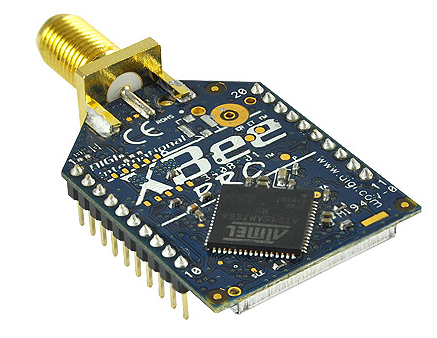
\includegraphics{figures/xbee.png}}
	\caption{}
	\label{fig:xbee}
\end{figure}

\subsubsection{IEEE 802.15.4 vezet�k n�lk�li protokoll}
\label{sect:prot}
Az IEEE\footnote{Institute of Electrical and Electronics Engineers}-nek egy csoportja a 802.15 mely a WPAN\footnote{Wireless Personal Area Network} h�l�zatok szabv�nyos�t�s�val foglalkozik, 7 alcsoportja k�z�l a 802.15.4 \cite{bib:ieee} a Low Rate WPAN nevet viseli. Ez a szabv�ny a kis fogyaszt�s�, olcs� �s alacsony s�vsz�less�g� vezet�k n�lk�li kommunik�ci�val foglalkozik. Az OSI modell els� (fizikai) �s m�sodik (adatkapcsolati) r�teg�t val�s�tja meg, erre �p�tkezik a ZigBee \cite{bib:zigbee} c�g �ltal specifik�lt protokoll verem.

A fizikai r�teg feladata fizikai �sszek�ttet�st teremteni a hardware-rel, specifik�lja, m�k�d�si fesz�lts�get, szab�lyozza a haszn�land� frekvenci�t, ami Eur�p�ban 868-868.6 MHz, �szak-Amerik�ban 902-928 MHz, vil�gszerte 2.4-2.4835 GHz-es ISM\footnote{Industrial, Scientific and Medical (ISM) s�vok, melyek szabadon haszn�lhat�ak ipari, tudom�nyos �s orvosi ter�leten } tartom�nyban helyezkedik el. Tov�bb� �tj�r�st biztos�t a felette l�v� adatkapcsolati r�tegnek, melynek feladata a hibamentes �tvitel biztos�t�sa 2 pont k�z�tt hibajav�t�ssal/jelz�ssel �s forgalomszab�lyz�ssal. A biteket keretekbe �gyazva k�ldi a fels�bb r�tegnek, maxim�lis m�rete 127 byte melynek form�tuma a IEEE 802.15.4-2011-ben van specifik�lva.

\begin{figure}[h]
	\centering
	\resizebox{5cm}{!}{
		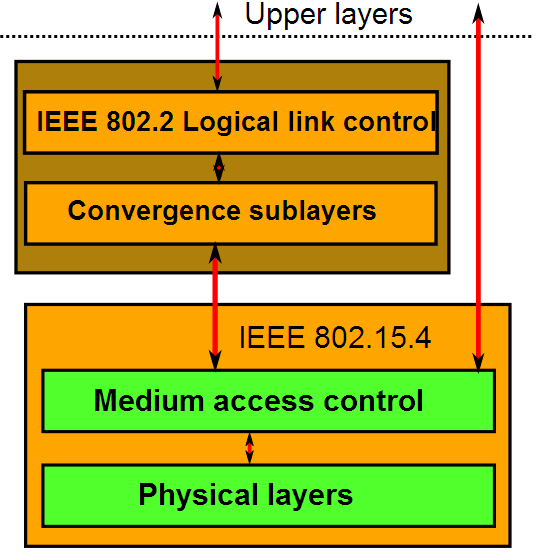
\includegraphics{figures/lrwpan.png}}
	\caption{}
	\label{fig:lrwpan}
\end{figure}

2 fajta topol�gia kialak�t�sa lehets�ges, egyik a pont-pont m�sik a csillag. Mindegyik eszk�z egy egy�ni 64 bites azonos�t�val rendelkezik.

A Zigbee 2 �jabb r�teget helyez az eddigiek f�l�, a h�l�zati �s az alkalmaz�sit, melybe beleker�lt a ZDOs\footnote{ZigBee Device Objects}, mely az eszk�z�k csatlakoz�s��rt, felder�t�s��rt �s biztons�g��rt felel�s.

\section{Saj�t feladat}

Feladatom k�z� tartozik a kapcsolat fel�p�t�se a rep�l�g�p �s a f�ldi �llom�s k�z�tt, melynek sor�n meg kell oldanom a soros porti kommunik�ci� l�trehoz�s�t �s a f�ggetlen adatok feldolgoz�s�t, kijelz�s�t. Ahhoz hogy a kialak�tand� megjelen�t�s felhaszn�l�bar�t legyen, t�bb n�zeti oldal sz�ks�ges: 
\begin{itemize}
\item Egy �ttekint� k�perny�, mely a legfontosabb adatokat jelen�ti meg a rep�l�vel kapcsolatban ( poz�ci�, sebess�g, ir�ny)
\item Egy tervez� modul, amin a lerep�lend� �tvonalhoz tartoz� fordul�pontok kijel�l�se lehets�ges
\item Egy diagnosztikai n�zet, melyen az alacsonyabb priorit�s� adatok tekinthet�ek �t
\end{itemize}


\subsection{Mi a f�ldi ir�ny�t� �llom�s feladata?} 

Egy UAV vezet�s�hez elengedhetetlen egy b�zis, ahonnan a f�ldi szem�lyzet ir�ny�tja, monitorozhatja a rep�l�st. �ltal�ban t�bb \cite{bib:aimofuav} funkci�t l�t el:
\begin{itemize}
\item K�ldet�s tervez�s: �tvonal meghat�roz�sa, illetve a c�lpontok kijel�l�se
\item K�ldet�s v�grehajt�s: t�vir�ny�t�ssal vezetve az oper�tor v�grehajtja a feladatot
\item Adatok megjelen�t�se: megfelel� m�don kijelezni a rep�l�g�p �llapot�t, esetleges hib�it
\end{itemize}


\subsection{Hibat�r� kommunik�ci� kialak�t�sa}

\subsubsection{Modem kommunik�ci�}

A modem soros port interface-t biztos�t, egy USB-RS232 �talak�t�val USB porton kereszt�l megoldhat� egy olyan sz�m�t�g�ppel is az �sszek�ttet�s, mely nem rendelkezik soros porttal, pl. saj�t energiaell�t�ssal rendelkez� modern laptop.

\subsubsection{P�rhuzamos csatorn�k}

Mivel a rep�l�g�pen duplik�ltak az elemek, �gy a k�ld� oldali modem is, a f�ggetlen jelek v�tel�re megold�st kell tal�lni �s az esetleges elt�r�sekkel sz�molni kell.

\subsubsection{Biztons�gos protokoll}

2 ir�ny� kommunik�ci� kialak�t�sa a c�l, �gy a k�ldend� adatok csomagj�nak biztons�gos protokollj�t ki kell dolgozni, mely az adatintegrit�s meg�rz�se �rdek�ben hibajelz�sre alkalmazhat�.

\subsection{Grafikus felhaszn�l�i fel�let}
asd


\section{F�ldi �llom�sok}

Sz�mos megold�s sz�letett f�ldi �llom�sok GUI\footnote{Graphics User Interface, grafikus megjelen�t�s}-jainak kialak�t�s�ra. Els�dleges k�vetelm�ny, hogy az oper�tor mindig a legfontosabb inform�ci�kat l�thassa, ehhez szoftverergon�miailag kell megtervezni a m�szerek. \cite{bib:multimodal} K�s�rleteket folytattak, milyen elrendez�sben, h�ny k�perny�n �rdemes megjelen�teni az adatokat, �gy, hogy az m�g ne terhelje t�l az oper�tort. Bebizonyosodott, hogy �rdemes t�bb �rz�kszerven kereszt�l jelz�seket adni, �gy pl. nagy priorit�s� esem�nyn�l a figyelmeztet� ablak megjelen�s�t hanghat�s is k�s�ri. Al�bbiakban �sszehasonl�t�sra ker�lnek a piacon l�v� megjelen�t�si fel�letek, megold�sok.


\subsection{ArduPilot}

Az \cite{bib:ardu} Ardupilot projekt l�trej�tt�nek oka, hogy otthoni k�r�lm�nyek k�z�tt, nem ipari alkatr�szekb�l b�rki �ssze�ll�thasson egy auton�m j�rm�vet, mely az el�re bet�pl�lt utas�t�sokat v�grehajtja. K�zponti eleme az Arduino c�g �ltal k�sz�tett ATMel mikroprocesszorra �p�tett platform, mely felhaszn�l�bar�tabb� teszi a mikroprocesszor programoz�s�t. Magas szint� utas�t�sokkal seg�ti az eszk�zzel val� bar�tkoz�st, nincs sz�ks�g assembly szint� tud�sra. Erre a platformra hozt�k l�tre az ArduPilot programot, k�pes vez�relni t�bbf�le auton�m j�rm�vet:
\begin{itemize}
\item ArduPlane n�ven fut� v�ltozat: robotrep�l�g�p
\item ArduCopter: 1, 3, 4, 6, 8, propelleres helikopter
\item Ardurover: 4 kerek� aut�
\end{itemize}
Sikeress�g�nek f� oka, a ny�lt forr�sk�d, Arduino panel alacsony �ra (~5 ezer Ft) �s a projekt m�g�tt �ll� lelkes k�z�ss�g.

Ennek a k�z�ss�gnek k�sz�nhet�en sz�letett a Mission Planner nev� szoftver, mely teljes k�r� t�mogat�st ny�jt a j�rm�vekkel kapcsolatban.


\subsubsection{F�k�perny�}

T�bb n�zet seg�ts�g�vel k�nnyen �tl�that� a funkcionalit�sa, rep�l�s szempontj�b�l a f�k�perny�n a legfontosabb adatok tal�lhat�ak. A rep�l�g�p orient�ci�j�t, sebess�g�t, ir�ny�t egy m�horizonton l�thatja a felhaszn�l�, ez vizu�lisan szeml�lteti, hogy h�ny fokos bed�nt�ssel rep�l, milyen �ll�ssz�ggel emelkedik. Alatta l�v� ter�leten el�re be�ll�tott adatokat jelen�t meg, pl. GPS magass�g, GPS sebess�g, sz�lir�ny( val�s m�gneses ir�ny �s a sebess�g vektor k�l�nbs�g�b�l sz�m�that�). A legnagyobb ter�letet a t�rk�p foglalja el, melyen az aktu�lis ir�ny, lerep�lt �tvonal, fordul�pontok l�that�ak. Megfigyelhet�, hogy ez kapja ar�nyaiban a legnagyobb ter�letet.

\begin{figure}[H]
	\centering
	\resizebox{15cm}{!}{
		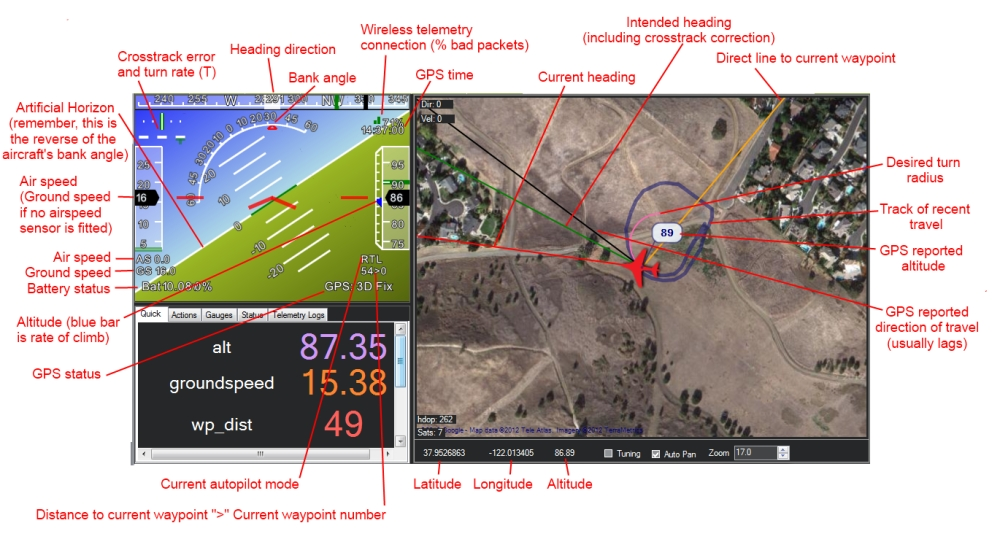
\includegraphics{figures/ardu.png}}
	\caption{}
	\label{fig:ardu}
\end{figure}

Ez a n�zet akkor j�het j�l, mikor olyan meghib�sod�s t�rt�nik, melyre nincs felk�sz�tve az ir�ny�t�egys�g �s sz�ks�ges lehet a k�zi �zemm�dra v�lt�s. El�fordulhat ilyen esetben, hogy nincs vizu�lis r�l�t�s az oper�tor �s a rep�l�g�p k�z�tt, ekkor csak az itt l�that� m�szerek �s t�rk�p alapj�n sz�ks�ges ir�ny�tania. Szerencs�re ez az avionik�ban m�r bizony�tott, hogy m�szerek seg�ts�g�vel, ``vakon'' is lehets�ges rep�lni, itt azonban ez az eset csak p�r percig sz�ks�ges.

\subsubsection{Tervez� �s �tvonalfelt�lt�}

M�sik n�zet lehet�s�get biztos�t �tvonalpontok kijel�l�s�re, az �tvonalpontokhoz egy list�b�l kiv�laszthat�, hogy az adott pont start-, fordul�-, v�gpont �s egy�b lehet�s�gek. Az �tvonalpontok poz�ci�j�t eg�rrel m�dos�thatjuk, t�r�lhetj�k. Bal fels� sarokban a kijel�lt tervnek hossz�t l�thatjuk, ez seg�ts�get ny�jt, nehogy t�lhaladjuk a r�di�kapcsolat �s a rep�l� hat�sugar�t. Az elk�sz�tett tervet felt�lthetj�k a csatlakoztatott eszk�zre.
\begin{figure}[H]
	\centering
	\resizebox{15cm}{!}{
		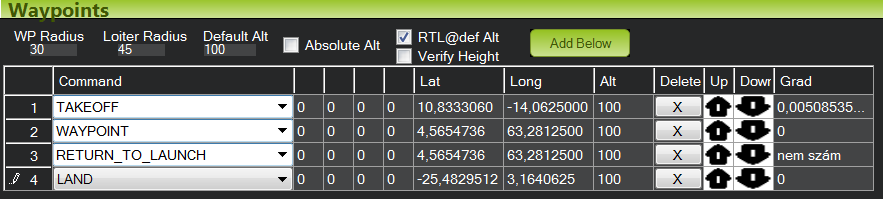
\includegraphics{figures/ardu_plan.png}} %plan
	\caption{}
	\label{fig:ardu_plan}
\end{figure}

\subsubsection{Be�ll�t�sok}

Itt lehet�s�g van a nyelv �s m�rt�kegys�gek kiv�laszt�s�ra, napl�z�s s�r�s�g�nek meghat�roz�s�ra.
Egy m�sik oldalon az aktu�lis j�rm�vet lehet be�ll�tani, mivel m�s adatok fontosak egy f�ldi �s egy l�gi j�rm� eset�ben, tov�bb� a kommunik�ci�s protokoll is v�ltoz�. Nem k�l�n oldalon, hanem mindig l�that� a csatlakoz�s gomb, melyn�l a soros port �s a jelsebess�g be�ll�t�sa ut�n a csalatkoz�s gombbal csatlakozik a program a portra.
\begin{figure}[H]
	\centering
	\resizebox{5cm}{!}{ 
		
\includegraphics{figures/ardu_conn.png}} %conn
	\caption{}
	\label{fig:ardu_plan}
\end{figure}
\subsubsection{Termin�l}

Ezen az oldalon az USB-n csatlakoztatott eszk�zt lehet parancssoron konfigur�lni. Az eszk�z saj�t LOG f�jljait let�lteni.

\subsubsection{Egy�b k�perny�k}

Lehet�s�g van m�g az elmentett log f�jlok szimul�l�s�ra, van egy s�g� oldal a program haszn�lat�val kapcsolatban, illetve egy t�mogat�i gomb, mely �tir�ny�t egy PayPal oldalra, ahol k�l�nb�z� �sszeggel t�mogathatjuk a fejleszt�st.


\subsubsection{�sszegz�s}

Felhaszn�l�i szempontb�l bar�ts�gos fel�letet biztos�t a k�l�nb�z� n�zetekkel, gombok �tgondolt elhelyez�s�vel.
Nem a program hib�ja, de nincs felk�sz�tve p�rhuzamos csatorn�k kezel�s�re, ez az ArduPilot projekt egyszer�s�g�nek k�sz�nhet�, mivel nem haszn�l redundanci�t. Mivel a rep�l�, melyhez a programot k�sz�tem, nagy megb�zhat�s�g�, �gy sz�ks�ges megoldani a 2 port kezel�s�t �s az azokon �rkez� adatok feldolgoz�s�t. J� �tlet a csatlakoz�s gomb mindig l�that� elhelyez�se, a f�k�perny�n t�rk�pen �br�zolni a rep�l� helyzet�t, illetve a m�horizont. Azonban hibadiagnosztikai kijelz�s nincs megoldva, melynek szint�n fontos a megval�s�t�sa.

\subsection{Paparazzi}
\cite{bib:paparazzi} Hasonl�an mint az ArduPilot, ez a projekt is a k�nnyen, otthon �sszeszerelhet� rep�l� meg�p�t�se jegy�ben sz�letett. Nem csak egy ny�lt forr�sk�d� robotpil�t�t ad, hanem komplett ``csin�ld magad'' k�szletet, melyben fesz�lts�gszab�lyz�t�l kezdve a GPS vev�ig mindent megkaphatunk. Tov�bb� a hozz� k�sz�lt f�ldi �llom�shoz antenn�t, modemet �s programot is ny�jt.

A program a k�vetkez� funkci�kkal rendelkezik:

\begin{itemize}
\item t�bb platform t�mogat�sa (fix- �s forg�sz�rny)
\item t�bb j�rm� egyidej� kezel�se
\item Google Maps, OpenStreetMaps, Microsoft Maps t�rk�pes megjelen�t�s
\item k�ldet�s tervez�s
\item mozgathat� ir�nypontok
\item val�sidej� fed�lzeti param�ter �ll�t�s
\item gyorsbillenty�
\item hangjelz�s
\item teljesen �tszabhat� grafikus fel�let
\end{itemize}


\subsubsection{F�k�perny�}

\begin{figure}[h]
	\centering
	\resizebox{15cm}{!}{ 
		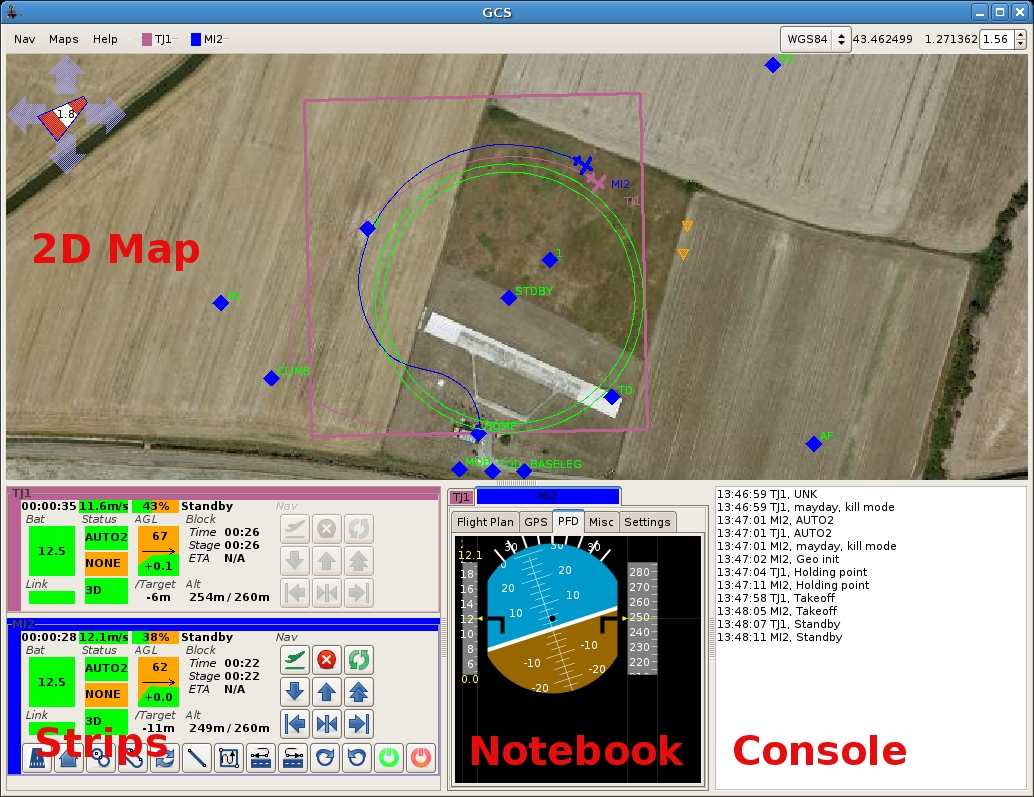
\includegraphics{figures/paparazzi.png}} %conn
	\caption{}
	\label{fig:paparazzi}
\end{figure}

\figref{paparazzi} �br�n l�that� k�perny� nagy sz�zal�k�t a t�rk�p foglalja el, melyen a lerep�lt �tvonal �s a fordul�pontok l�that�ak. A rep�l� aktu�lis helyzete mellett a neve, sebess�ge �s rep�l�si magass�ga is kijelezve van. Bal oldalt egy inform�ci�s s�vban a k�vetkez� fontosabb adatok l�that�ak: akkumul�tor t�lt�tts�ge, sebess�g, tol�er�, magass�g, illetve utas�t�sok: fel-, lesz�ll�s, megfigyel�s ind�t�sa. Jobb fels� sarokban a kurzor t�rk�pen l�v� koordin�t�ja ker�l megjelen�t�sre. 


A t�rk�pet a k�k nyilakra val� kattint�ssal �s a billenty�zet nyilainak lenyom�s�val lehet mozgatni, nagy�tani az eg�r g�rg�j�vel �s a ``Page up/down'' gombokkal. Az \textbf{f} gomb megnyom�s�val az �sszes fordul�pont l�that� a k�perny�n. A fordul�pontokat is ezen a fel�leten lehet szerkeszteni. A m�dos�t�sok egy meger�s�t� �zenet j�v�hagy�sa ut�n t�lt�dnek fel a rep�l�re, melyre az egy meger�s�t� v�lasszal reag�l. �jat csak felsz�ll�s el�tt lehets�ges felt�lteni.

K�z�pen alul tal�lhat� egy t�bb f�llel ell�tott r�sz, melyn�l kiv�laszthat�, hogy �ppen egy m�horizontot, a GPS �ltal vett adatokat, az �tvonaltervet vagy a be�ll�t�sokat szeretn�nk-e l�tni.

\subsubsection{�sszegz�s}
Itt sem l�tfontoss�g� t�nyez� az elemek redundanci�ja, �gy nincs felk�sz�tve egy j�rm�b�l �rkez� p�rhuzamos jelek fogad�s�ra. Egy k�perny� szolg�l a navig�ci�ra �s az �tvonal-kijel�l�sre, mely szerintem nem a legjobb megold�s. �sszess�g�ben ez is egy nagyon j�l haszn�lhat� program, mely teljesen kiszolg�lja az UAV-kat melyhez k�sz�tett�k

\subsection{MicroPilot Horizon}

\cite{bib:makkay} ``Az 1995 �ta m�k�d� kanadai \cite{bib:micropilot} MicroPilot a vil�g egyik legismertebb robotpil�ta gy�rt� c�ge, 65 orsz�gban t�bb mint 750 alkalmaz� haszn�lja az eszk�zeiket. N�pszer�ek az iskol�kban, egyetemeken, kutat� int�zetekben, a gazdas�g k�l�nb�z� ter�letein, de a v�delmi szf�ra is sz�p sz�mmal haszn�l robot l�gi j�rm�vein MicroPilot berendez�seket. Az adat�tviteli csatorna ugyanazokat a funkci�kat k�pes biztos�tani, mint a programbeviteln�l haszn�lt k�beles �sszek�ttet�s, �gy ezen kereszt�l rep�l�s k�zben is m�dos�that� az �tvonal, a rep�l�si param�terek �s az egy�b be�ll�t�sok. A MicroPilot fed�lzeti egys�ge ezen k�v�l egy r�di� t�vir�ny�t� (RCON) vev�berendez�st is fogad, amely lehet�s�get teremt a f�ldi ad� konzolj�r�l az ir�ny�t�s �tv�tel�re �s botkorm�nyos k�zi vez�rl�sre. Ezt alapvet�en a fel �s lesz�ll�s idej�re, illetve az �tvonal kritikus szakaszain haszn�lj�k. Amennyiben az RC t�vir�ny�t�val m�k�d� rep�l�g�p veszti el a kapcsolatot, akkor a fed�lzeti vev�berendez�s FAILSAFE �zemm�dra kapcsol �s annak be�ll�t�sa szerint m�k�dteti a rep�l�g�pet. A FAILSAFE vagy az utols� szervo �ll�st �rzi meg, vagy egy el�re programozott legbiztons�gosabb f�ldet �r�st �g�r� be�ll�t�sra ugrik.''
A hozz� k�sz�tett f�ldi ir�ny�t� egys�g a MicroPilot Horizon nevet viseli. 
\begin{figure}[h]
	\centering
	\resizebox{10cm}{!}{ 
		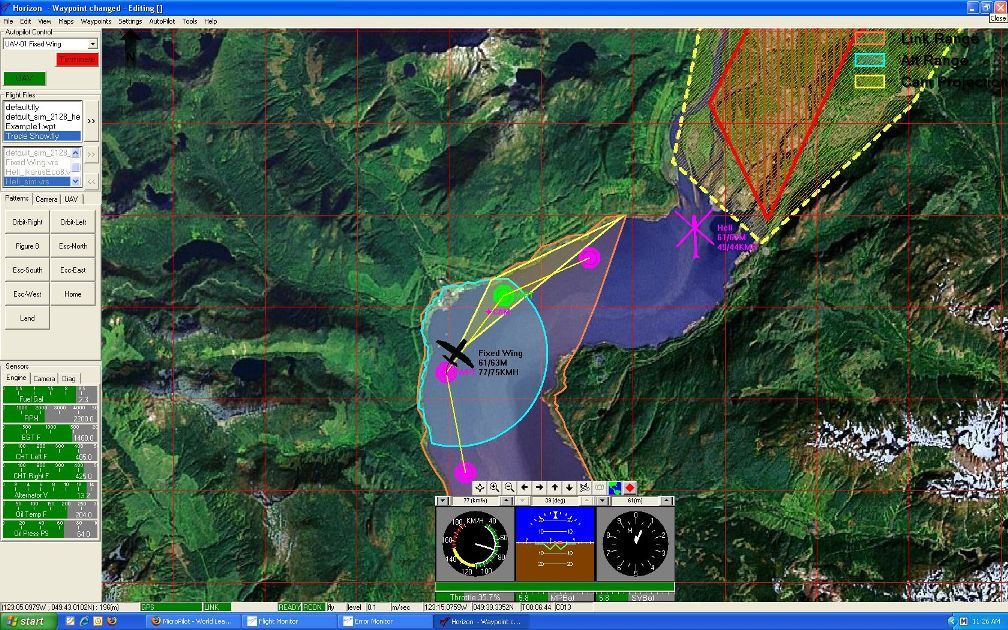
\includegraphics{figures/micropilot.png}} 
	\caption{}
	\label{fig:micropilot}
\end{figure}
T�bbek k�zt a k�vetkez� tulajdons�gok jellemzik:

\subsubsection{Biztons�g}

A t�rk�pen kijel�lhet�ek azok a ter�letek, ahova nem szabad berep�lni, ha a k�zel�be ker�lne a rep�l�, figyelmeztet�st kap az oper�tor. Automatikus tengerszint feletti magass�g  �s lesz�ll�hely be�ll�t�s, arra az esetre, ha a kapcsolat megszakadna a f�ldi ir�ny�t�ssal.

\subsubsection{Oper�tor k�zpont�s�g}

Rep�l�si terv k�nnyen, kattint�ssal �ssze�ll�that� �s m�dos�that�, mind rep�l�s el�tt �s k�zben. POI\footnote{Point Of Interest, �rdekes hely mely GPS koordin�t�val megjel�lhet�} gombnyom�sra lerakhat� a t�rk�pen, a j�v�beni kivizsg�l�shoz. Vonalz� eszk�z seg�ts�g�vel k�nnyen v�gezhet sz�m�t�st az �tvonal hossz�val kapcsolatban. Gazdag online s�g�ja gyorsan v�laszt ad a k�rd�sekre.

\subsubsection{T�bb eszk�z egyidej� kezel�se}

T�bb eszk�zh�z tud egyszerre csatlakozni �s kiszolg�lni, legyen az rep�l� vagy helikopter, mindegyikhez k�l�n n�v rendelhet�. Az �sszes csatlakoztatott j�rm� k�z�tt szinkroniz�lva vannak az �tvonalpontok, egy-t�bb �s t�bb-t�bb topol�gia kialak�t�s�ra is van lehet�s�g.

\subsubsection{Szimul�ci�}

M�r a legels� kiad�sn�l r�j�ttek a szimul�ci� jelent�s�g�re, mivel ezzel a megold�ssal a legegyszer�bb a j�v�beli oper�torok kik�pz�se. Lehet�s�g van minden platform szimul�l�s�ra SIL m�dban.

\subsubsection{Kamera}

A rep�l�g�pre szerelt kamera k�p�nek megjelen�t�se kulcsfontoss�g�, mivel a kezel� ezzel l�thatja legink�bb a rep�l�g�p helyzet�t �s a megfigyelt c�lpontot. MPEG4 t�m�r�t�s cs�kkenti a sz�ks�ges s�vsz�less�get. Ebben a m�dban a legfontosabb rep�l�ssel kapcsolatos inform�ci�k �tl�tsz�an jelennek meg, �gy nem kell m�sik k�perny�re tekintenie a kezel�nek.


\subsubsection{Figyelmeztet�s}

K�l�nb�z� hib�k l�phetnek fel rep�l�s k�zben, ezeket egy napl�ban t�rolja a program. Lehet�s�g van k�l�nb�z� priorit�si szintek meghat�roz�s�ra, hangjelz�s hozz�rendel�s�re. �gy egy bizonyos szint alatti hib�k nem terelik el az oper�tor figyelm�t.

\subsubsection{Telemetrikai adatok megjelen�t�se}

15 �rz�kel� adatait tudja grafikusan �br�zolni, elmenteni, bet�lteni. Statisztikai anal�zist biztos�t, �tlag, minimum, maximum keres�sre. Kiugr� �rt�keket pirossal megjel�l, hogy k�nnyen �szrevehet� legyen egy jel hat�ron k�v�li �rt�ke.

\subsubsection{�sszegz�s}

Ez a program els�sorban t�vir�ny�t�sos �zemm�d t�mogat�s�ra k�sz�lt, mely sor�n az oper�tor ir�ny�tja a g�pet �s ehhez a legt�bb inform�ci�t szolg�ltatja. �gy kulcsfontoss�g� a vide�k�p �tvitel t�mogat�sa �s a legfelhaszn�l�bar�tabb megjelen�t�s.



%http://www.szrfk.hu/rtk/folyoirat/2013_1/2013-1-04-Imre_Makkay.pdf
%http://www.szrfk.hu/rtk/kulonszamok/2012_cikkek/77_Makkay_Imre-Papp_Timea.pdf
%http://www.unmannedgroup.com/index.php?page=2&subpage=6&data=9
%http://www.uavfactory.com/product/16


\subsection{OpenPilot}
\cite{bib:openpilot} A projekt c�lja, hogy ny�lt forr�sk�d�, magas min�s�g� robot pil�t�t hozzanak l�tre auton�m rep�l�kh�z. 2009-ben alakult, az�ta m�r t�bb mint 200 tagja vesz r�szt a fejleszt�sben a vil�g 140 orsz�g�b�l. A jelenlegi verzi�, k�pes ir�ny�tani fix sz�rnyas rep�l�t �s helikoptert 2-t�l 8 rotorig. 
A robotpil�ta egy Cortex-M3 32 bit ARM 72MHz mikrokontrollerre �p�l, 3 szabads�gi fokos gyorsul�s�rz�kel�vel �s ir�nyt�vel, GPS vev�vel, 12 bites A/D �talak�t�val a m�rt �rt�kek digitaliz�l�s�ra.

A hozz� k�sz�lt GCS t�bb platformon m�k�dik: Windows, Mac OS, Linux, tervben van az Android t�mogat�s is. Seg�ts�g�vel t�lthet� fel a panelra a fed�lzeti program, illetve interface-t biztos�t a rep�l�s alatt.

\subsubsection{F�k�perny�}

Bal oldalon m�horizont l�that�, alatta az aktu�lis j�rm� orient�ci�ja k�ls� n�zetb�l, jobb oldalon a t�rk�p az aktu�lis poz�ci� megjelen�t�s�vel.

Ez a n�zet szabadon m�dos�that�, k�l�nf�le ``gadget''-ek kiv�laszt�s�val, pl. a k�ls� n�zet helyett egy m�rt �rt�k grafikus megjelen�t�s�re kicser�lhet�. Ezek .xml f�jlba elmenthet�ek �s visszat�lthet�ek, k�l�nb�z� konfigur�ci� ig�nyeihez igazodva.


\begin{figure}[H]
	\centering
	\resizebox{15cm}{!}{ 
		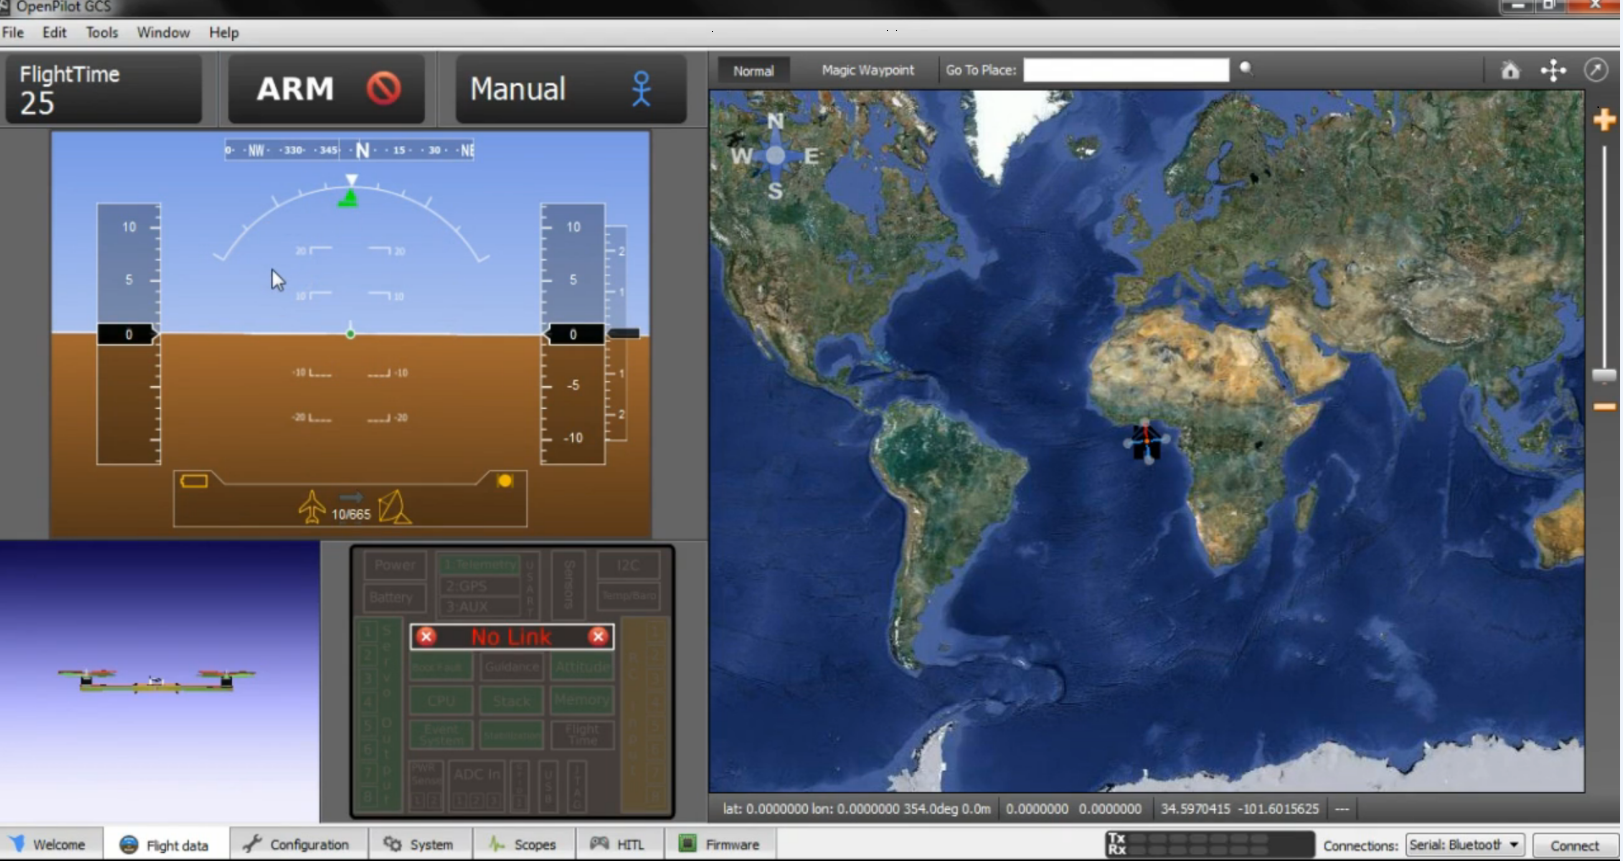
\includegraphics{figures/openpilot.png}} 
	\caption{}
	\label{fig:openpilot}
\end{figure}


\subsubsection{Be�ll�t�sok}

Itt �ll�that�ak be a kommunik�ci�s portok, az akt�lis j�rm� t�pusa, a t�rk�p megjelen�t�se, a szerv� motorok semleges helyzete.

\subsubsection{Telemetria}

A fogadott adatokat t�bbf�lek�ppen meg tudja jelen�teni. Lehets�ges a kiv�lasztottakat egy sk�l�n egyszerre kirajzolni, vagy k�l�n-k�l�n grafikonokon.

\subsubsection{�sszegz�s}
Rengeteg be�ll�t�si lehet�s�get ny�jt ez a program, lelkes k�z�ss�g �ll m�g�tte, minden olyan fontos elv�r�st kiel�g�t, mely napjainkban felmer�lhet egy UAV adatainak megjelen�t�s�vel kapcsolatban.

\subsection{QGroundControl}
\cite{bib:qground} 


\begin{figure}[H]
	\centering
	\resizebox{15cm}{!}{
		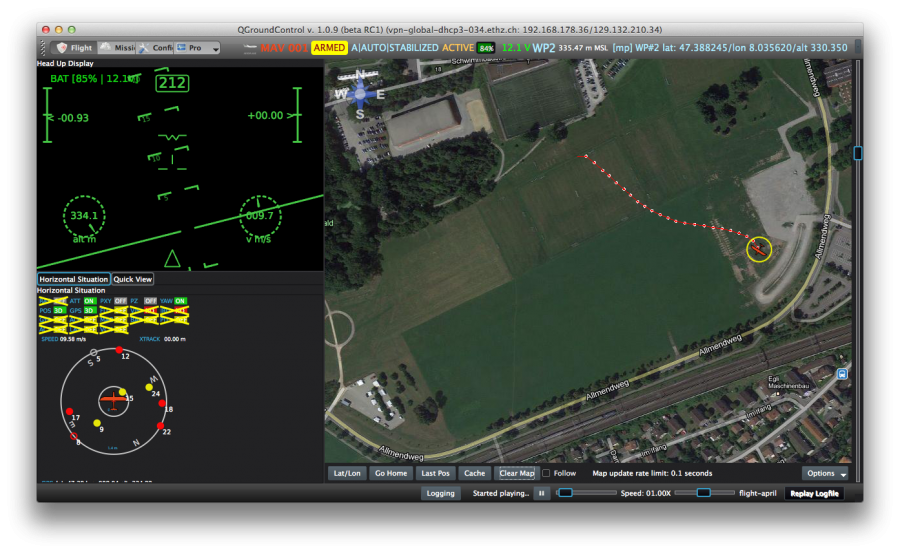
\includegraphics{figures/qground.png}}
		\caption{}
	\label{fig:qground}
\end{figure}



\subsection{�sszehasonl�t�s}

A felsorolt megold�sok �sszehasonl�t�s�b�l kider�l, hogy egyik sem alkalmaz redundanci�t a kommunik�ci� megval�s�t�s�ra. Az �sszesre jellemz�, a poz�ci� t�rk�pen t�rt�n� vizualiz�ci�ja.

\begin{table}
	\begin{center}
			\begin{tabular}{| l | l | l | l |}
				\hline
				Program		 			& Forr�sk�d 				& El�ny 				& H�tr�ny 					  \\ \hline
				Ardupilot				& C\#, ny�lt 				& 						  & nincs redundancia	 	\\ \hline
				Paparazzi 			& ?, nem ny�lt			&								& nincs redundancia	 	\\ \hline
				MicroPilot 			& 									&								& nincs redundancia	 	\\ \hline
				QGroundControl 	& C++, ny�lt				&								& nincs redundancia	 	\\ \hline
			\end{tabular}
	\end{center}
	\caption{�sszefoglal�s}
	\label{tab:up}
\end{table}

%----------------------------------------------------------------------------
\chapter{Tervez�s}
%----------------------------------------------------------------------------
\section{Kommunik�ci�}

A kommunik�ci� csatorn�nk�nt 2 db modem seg�ts�g�vel t�rt�nik, a modemek egym�s k�zt vezet�k n�lk�l csatlakoznak, felhaszn�l�i oldalon soros portot biztos�tanak. �gy az elk�sz�tend� programnak el�g csak a soros port jeleinek v�tel�vel foglalkoznia. A modemek adat�tviteli sebess�ge v�ltoz� lehet, �gy azt a felhaszn�l� egy list�b�l v�laszthatja csatlakoz�s el�tt. �talak�t�val lehet�s�g adatik USB-n kereszt�l soros port megval�s�t�s�ra, �gy k�nnyen kezelhet�v� v�lik a perif�ria illeszt�s

\section{Adatok fogad�sa}

A redundanci�b�l k�vetkez�en k�l�n, k�l�n kell kezelni a 2 p�rhuzamos csatorn�n kapott adatokat. Mivel aszinkron m�don �rkeznek a csomagok, �gy kett� t�rol� kell, mely a legut�bb k�ld�tteket t�rolja egy FIFO list�ban.

\subsection{Protokoll}

Az adatokat a rep�l�g�p 2 Hz-s frekvenci�val k�ldi, ezek csomagokban �rkeznek, melyeknek a fel�p�t�se:

\begin{figure}[H]
 \hspace*{-3cm}  
	\resizebox{20cm}{!}{
		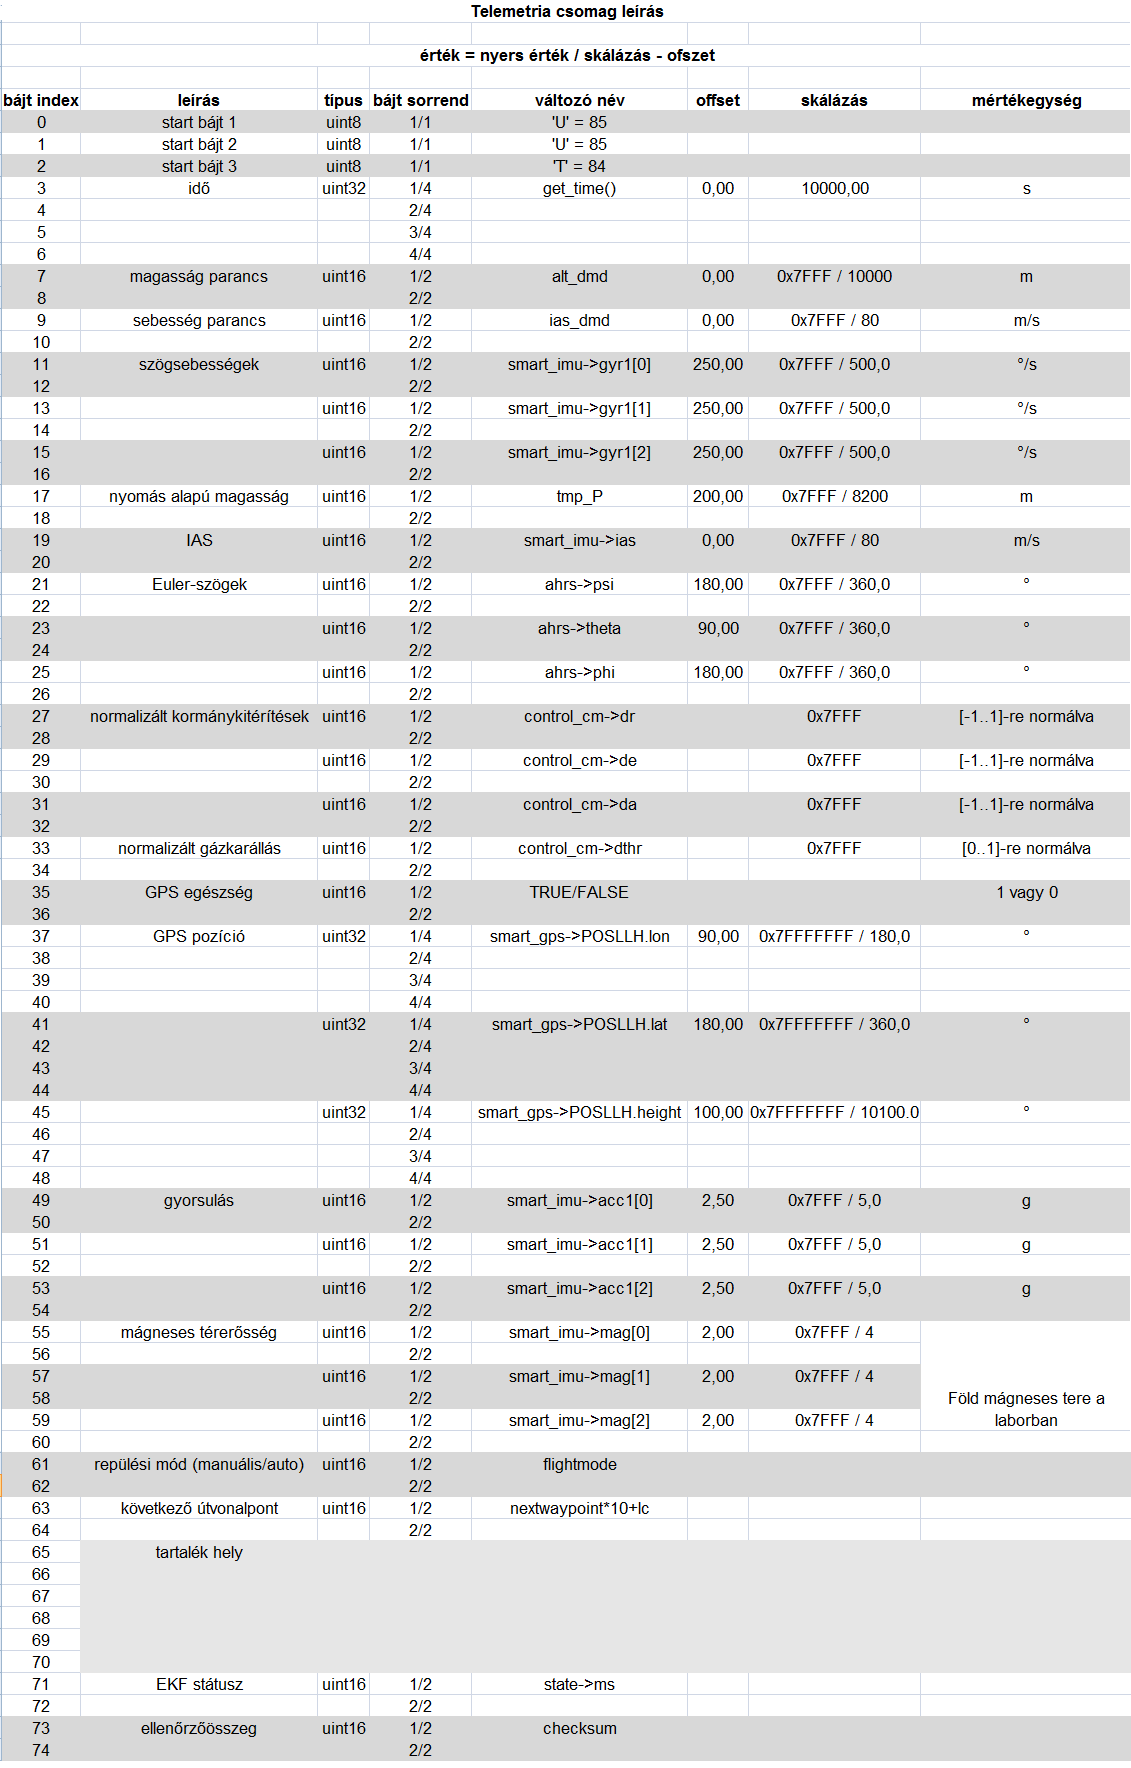
\includegraphics{figures/downprot.png}}
\end{figure}


%\begin{table}[H]
%\begin{center}
%		\begin{tabular}{| l | l | l | l |l |}
%			\hline    b�jt index 	& le�r�s 				& t�pus & sk�l�z�s 		       & offset \\ \hline
%				1 					& start 				& char(fix 'U') &   					       &    						 \\ \hline
%				2 					& start 				& char(fix 'U') &   					       &    						 \\ \hline
%				3						& start 				& char(fix 'T') &   					       &    						 \\ \hline
%				4 					& id�  					& uint32 				& 10000 			       & 0  						 \\ \hline
%				8 					& magass�g 			& uin16 				& 0x7fff/1000	       &    						 \\ \hline
%				\dots 			&   						&   						&   					       &    						 \\ \hline
%				\dots 			&   						&   						&   					       &    						 \\ \hline
%				\dots 			&   						&   						&   					       &    						 \\ \hline
%				\dots 			&   						&   						&   					       &    						 \\ \hline
%				\dots 			&   						&   						&   					       &    						 \\ \hline
%				\dots 			&   						&   						&   					       &    						 \\ \hline
%				\dots 			&   						&   						&   					       &    						 \\ \hline
%				\dots 			&   						&   						&   					       &    						 \\ \hline
%				\dots 			&   						&   						&   					       &    						 \\ \hline
%				\dots 			&   						&   						&   					       &    						 \\ \hline
%				\dots 			&   						&   						&   					       &    						 \\ \hline
%				\dots 			&   						&   						&   					       &    						 \\ \hline
%				TODO & �szaki ir�ny 1/2 	& unsigned short & 0x7FFF/400 &  200 \\ \hline
%				28 & keleti ir�ny 1/2 & unsigned short & 0x7FFF/400 &  200 \\ \hline
%				30 & lefel� ir�ny 1/2 & unsigned short & 0x7FFF/400 &  200 \\ \hline
%			
%				\dots &   &   &   &    \\ \hline
%			\end{tabular}
%\end{center}
%	\caption{Fogad�s protokollja}
% \label{tab:down}
%\end{table}

A sk�l�z�s �s offset k�pz�s az�rt sz�ks�ges, hogy az adott sz�less�gen (8, 16, 32 bit) min�l t�bb biten legyen �br�zolva egy �rt�k, mivel kis v�ltoz�sok eset�n a Hamming-t�vols�g\footnote{Bin�ris sz�mok XOR k�pz�s�vel kapott 1-esek sz�ma} kicsi lenne az eredeti sz�m�br�zol�son. Ahol sz�ks�ges, ott a  visszak�dol�s az al�bbi form�ban t�rt�nik : \\
$eredeti  = (nyers adat/skalazas) - offset $ \\
Az �rt�kek megfelel� kiv�laszt�sa a min�l nagyobb sz�tsz�r�shoz sz�ks�ges.

\section{Adatok k�ld�se}

A rep�l�g�p �ltal lerep�lend� feladat �tvonalpontjait hasonl�k�ppen, mint az adatok fogad�s�t, vezet�k n�lk�li csatorn�n k�ldj�k fel. A felt�ltend� adat k�ld�s�nek protokollja l�tfontoss�g�, mivel ha valamilyen hiba ker�l a kommunik�ci�ba akkor az ak�r v�gzetes is lehet. Gondolok itt olyan hib�ra, hogy egy fordul�pont koordin�t�ja �gy ker�l felt�lt�sre, hogy az kiesik a rep�l� hat�sugar�b�l �s ezzel nem sz�molva, lemer�l a t�pell�t�st szolg�l� akkumul�tor. Az ilyen hib�k ellen c�lszer� a felt�lt�s protokollj�ba hibadetekt�l�st �p�teni, hogy ezek a feldolgoz�s el�tt der�ljenek ki.

Felmer�l a k�rd�s, hogy a k�ld�s mikor enged�lyezett, a felsz�ll�s el�tt vagy rep�l�s k�zben is? L�thattuk n�h�ny megold�sban, hogy lehet�s�g van az �tvonal m�dos�t�s�ra menet k�zben is, ez egy j� opci�, �gy �rdemes ezt is megval�s�tani. Egyetlen probl�ma ennek mik�ntje, ha csak egy pont koordin�t�j�t m�dos�tjuk, akkor csak ezt vagy az �sszeset k�ldj�k? Ennek egyik megold�sa az lehet, hogy korl�tozzuk az el�sz�r felt�lt�tt pontok sz�m�ra �s az �sszes pontot �jra elk�ldj�k. A m�dos�t�s feldolgoz�s�t r�b�zzuk a fed�lzeti implement�ci�ra, hogyha egy ponton �thaladt, akkor az ut�lag hi�ba lett m�dos�tva, a k�vetkez� fordul�pont fel� halad. Tov�bbi strat�gi�k is elk�pzelhet�ek, de a tov�bbi fejezetekben taglaltak miatt, ezt �rdemes v�lasztani.

\subsection{Protokoll}

T�bb megold�s is lehets�ges a fordul�pontok felt�lt�s�re:
\begin{itemize}
\item R�gz�tett maxim�lis darabsz�m elk�ld�se egy csomagban
\item V�ltoz� darabsz�m eset�n egy fordul�pont egy csomagban
\end{itemize}


Az els� megold�sban r�gz�ten�nk a fordul�pontok maxim�lis sz�m�t. Mely azt eredm�nyezn�, hogy egy csomagban el lehetne k�ldeni az eg�sz lerep�lend� feladatot. Ha egy pont koordin�t�j�nak �br�zol�s�ra el�g 2*4 byte, �gy ha felt�telez�nk egy 10 pontot tartalmaz� (10*2*4 byte adat) csomagot, akkor annak m�rete fejl�ccel (3 b�jt), checksum mez�vel (2 b�jt) 79 b�jt. Ehhez hozz�j�nne m�g a pontok sz�ma, mely a fogad� oldali feldolgoz�st seg�ten�, ennek m�rete 1 b�jt.


M�sik lehet�s�gn�l b�rmennyit (N db) lehetne felt�lteni: egy csomag szerkezete: fejl�c, k�ldend� pontok sz�ma, aktu�lis pont sorsz�ma, koordin�t�i, checksum. Ha a  k�ldend� pontok sz�ma �s az aktu�lis pont sorsz�ma megegyezik �s meg�rkezett minden csomag akkor ACK-val v�laszol ha k�sz a felt�lt�s. Ez hibakezel�s szempontj�b�l kedvez�bb, mivel ha egy pont sorsz�ma nem egyezik meg az elv�rttal, akkor �jrak�ld�s k�r�s�vel el�g csak az adott pont �jrak�ld�s�vel terhelni a csatorn�t.

Mivel az eddig haszn�lt megold�sban a k�dba ,,bele volt �getve'' az �tvonalterv, mely 5-6 pontot tartalmazott, az els� megold�s t�nik kedvez�bbnek. Fogad� oldalon is k�nnyebb egy ilyen lehet�s�gre felk�sz�teni. Ha esetlegesen a j�v�ben t�bb fordul�pontont felt�lt�s�re lesz ig�ny, az is megoldhat� m�dos�t�sokkal.

A felt�lt�s sor�n mindkett� csatlakoztatott modem seg�ts�g�vel redund�nsan k�ldj�k el az el��ll�tott csomagot. Ha a csomag s�rtetlen�l meg�rkezett, ACK jelz�ssel v�laszolnak, melyet fogadunk �s visszajelezz�k a kezel�nek.

Egy 80 b�jtos csomag tartalma:
\begin{table}
	\begin{center}
			\begin{tabular}{| l | l | l | l |l |}
				\hline
				b�jt index 	& le�r�s 				& t�pus 				& sk�l�z�s 		& offset  \\ \hline
				0 					& start 				& b�jt(fix 'G') &   					&    			\\ \hline
				1 					& start 				& b�jt(fix 'P') &   					&    			\\ \hline
				2						& start 				& b�jt(fix 'S') &   					&    			\\ \hline
				3 					& pontok sz�ma	& b�jt    			& 			 			&    			\\ \hline
				4 					& pontok[0].lat & uin32 				& 0x7fff/360	&  180		\\ \hline
				\dots 			&   						&   						&   					&    			\\ \hline
				8 					& pontok[0].lon & uin32 				& 0x7fff/360	&  180		\\ \hline
				\dots 			&   						&   						&   					&    			\\ \hline
				12 					& pontok[1].lat & uin32 				& 0x7fff/360	&  180		\\ \hline
				\dots 			&   						&   						&   					&    			\\ \hline
				16 					& pontok[1].lon & uin32 				& 0x7fff/360	&  180		\\ \hline
				\dots 			&   						&   						&   					&    			\\ \hline
				78 					& checksum 1/2	& uin16 				& 						&  				\\ \hline
				79 					& checksum 2/2 	& uin16 				& 						&  				\\ \hline

			\end{tabular}
	\end{center}
	\caption{K�ld�s protokollja}
	\label{tab:up}
\end{table}

Felmer�lhet a k�rd�s, hogy a felt�lt�s ezzel a protokollal el�g hibat�r�-e, mivel a fogad�s protokollja is hasonl�an van megoldva, �gy el�gs�gesnek t�nik. Mivel ha a k�ld�s megfelel�en lezajlott, kapunk visszajelz�st, ha nem akkor lehet�s�g van az �jb�li elk�ld�sre.

\section{Grafikus fel�let}

Az el�z� fejezetben ismertetett grafikus fel�letekb�l levonva a k�vetkeztet�seket, nyilv�nval�, hogy a GUI kialak�t�s�ban fontos a rep�l�g�p aktu�lis poz�ci�j�nak t�rk�pen val� mutat�sa, az rep�l�si �llapot k�nnyen �rtelmezhet� megjelen�t�se, illetve az esetlegesen el�fordul� probl�m�k felt�n� jelz�se.

\subsection{F�k�perny�}

A f�k�perny�n l�that� lesz a rep�l�g�p aktu�lis poz�ci�ja �s ir�nya. A pozicion�l�st seg�tend�, egy t�rk�p lesz egy rep�l�g�p ikon h�tter�ben. Ez a r�sz a k�perny� kb. 2/3-�t fogja elfoglalni. Az oldals� s�vban a ``Glass Cockpit'' ker�l kialak�t�sra, ez a n�zet tartalmazza a g�p aktu�lis sebess�g�t, ir�nyt� seg�ts�g�vel ir�ny�t, magass�g�t, emelked�s�nek sebess�g�t. Val�sz�n�leg ez a k�perny� lesz legnagyobb sz�zal�kban haszn�lva, �gy a kritikus hib�kr�l itt kell felt�n� �rtes�t�st adni. Melyet a h�tt�rben dolgoz� hibadetekt�l� algoritmus v�lt ki. Az �rtes�t�s egy felugr� ablak lenne, mely tartalmazza, mely �rt�k hib�j�b�l keletkezett.

\subsection{Tervez�s k�perny�}

Ezen a k�perny�n a felhaszn�l� kijel�lheti a lerep�lend� �tvonalhoz tartoz� fordul�pontokat, melyet csatlakoz�s ut�n aszinkron m�don felt�lthet a rep�l�re. Mivel a kommunik�ci�s protokoll 10 pontot enged meg, �gy enn�l t�bbet itt ki sem jel�lhet, a lerakott pontok hely�t a megszokott Google Maps-hoz hasonl� m�don hosszan kattintva �trakhat�nak kell lennie, illetve k�ztes pontoknak t�r�lhet�eknek kell lenni�k. L�thattuk, hogy �rdemes a kijel�lt �tvonal hossz�r�l t�j�koztatni a felhaszn�l�t, �gy ez egy hasznos funkci�.

\subsection{Diagnosztikai k�perny�}

A 2 porton �rkez� dek�dolt �rt�kek l�tsz�dn�nak 2 oszlopban, mellett�k egy hiba�rt�k, mely a k�l�nb�z� hibat�pusok hibasz�m�nak �sszege lenne. 

\subsubsection{Hibat�pusok}
\begin{itemize}
\item beragad�s
\item t�l nagy v�ltoz�s
\item t�l nagy k�l�nbs�g a 2 vett �rt�ken
\end{itemize}

Ezek feldolgoz�s�ra 2 FIFO sort kell alkalmazni, melyek visszamen�leg t�rolj�k a be�rkez� �rt�keket. Ez az�rt sz�ks�ges, mivel �gy a t�ls�gosan kiugr� �rt�keket detekt�lni lehet, illetve, ha az eg�sz sorban ugyanazok az �rt�kek vannak, gyan�s a beragad�s es�lye.
A harmadik esetben sajnos nem lehets�ges a ``j�'' kiv�laszt�sa, mivel nem tudjuk, melyik modemb�l �rkezett adat a megfelel�. Ezt csak h�romszoroz�ssal �s t�bbs�gi szavaz�ssal lehetne megoldani. �gy a kett� �rt�k �tlag�t lehet csak felhaszn�lni.

\subsection{Termin�l k�perny�}

Lehet�s�g ny�lik a fogadott csomagok hexadecim�lis form�ban t�rt�n� megjelen�t�se, �gy az oper�tor alacsony szinten megbizonyosodhat a kapcsolat l�trej�tt�ben, mivel l�thatja a csomagok fel�p�t�s�t. Ha a fejl�c a csomag elej�n l�tsz�dik, akkor m�k�dnie kell a tov�bbi dek�dol�snak, melyet a t�bbi n�zet haszn�l fel. Ha nem l�tna itt adatokat, akkor ellen�rizheti, hogy val�ban j� portot illetve adatsebess�get v�lasztott-e ki.

%----------------------------------------------------------------------------
\chapter{Megval�s�t�s}
%--------------------------------------

\section{F�k�perny�}

\begin{figure}[H]
	\centering
	\resizebox{15cm}{!}{
		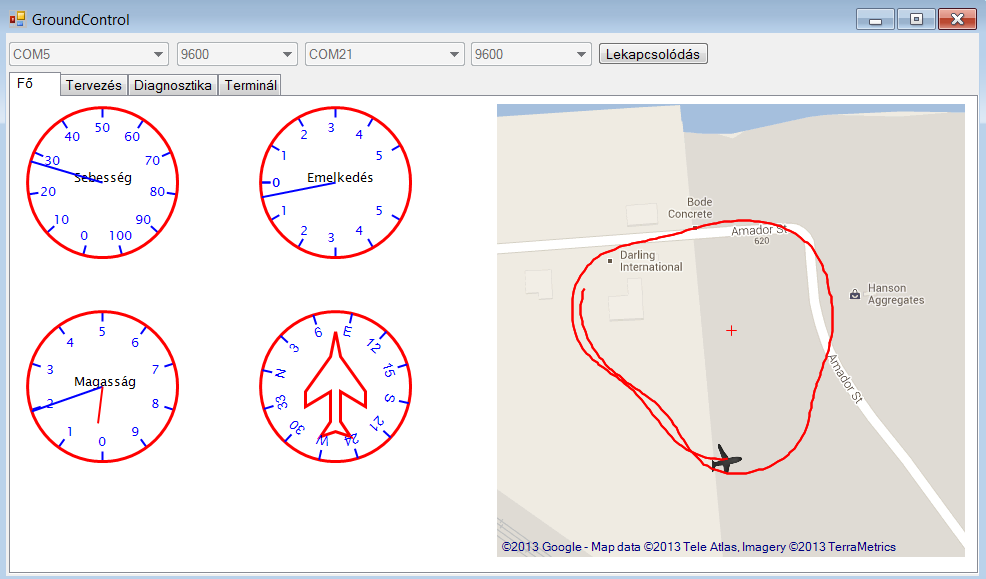
\includegraphics{figures/fokepernyo.png}}
	\caption{}
	\label{fig:fokepernyo}
\end{figure}

\section{Tervez�s k�perny�}

\begin{figure}[H]
	\centering
	\resizebox{15cm}{!}{
		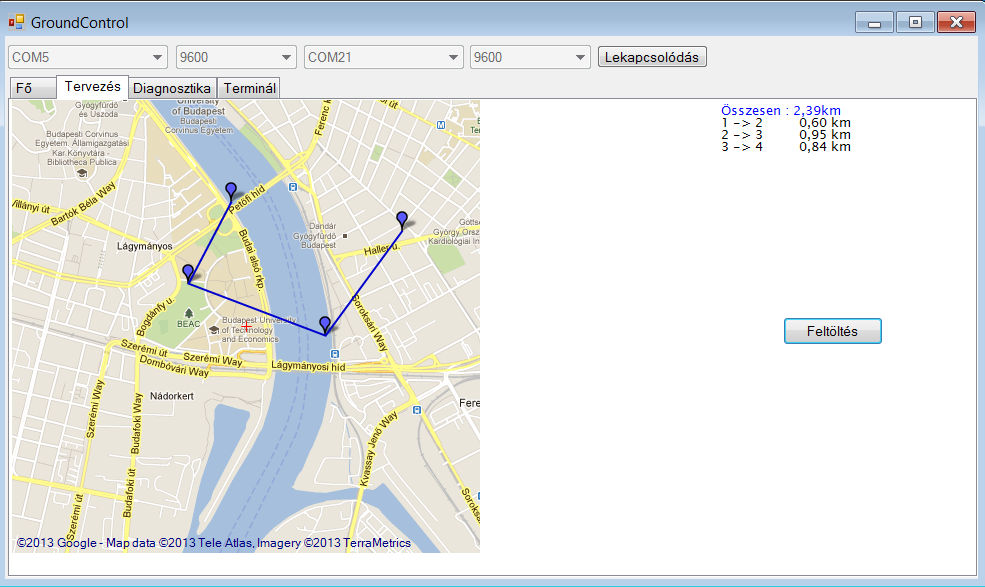
\includegraphics{figures/tervkepernyo.png}}
	\caption{}
	\label{fig:tervkepernyo}
\end{figure}

\section{Hibadiagnosztika}


\section{RS232}
A modemb�l �rkez� adatokat soros porton kereszt�l fogadja a program, a tesztk�rnyezet fel�ll�t�s�hoz HIL adatok szolg�ltak. A k�ld�tt log f�jlokat egy programmal beolvasom �s egy \cite{bib:null}null-modem seg�ts�g�vel sorosporton kereszt�l k�ld�m a megfelel� portra. 

\begin{figure}[!ht]
	\centering
	\resizebox{10cm}{!}{
		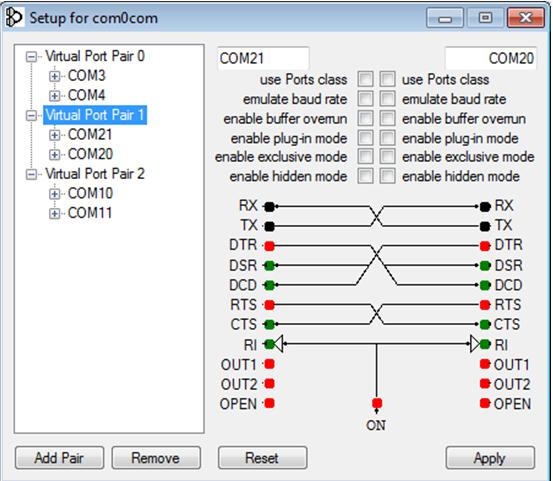
\includegraphics{figures/comnull.png}}
	\caption{}
	\label{fig:comnull}
\end{figure}

Be�ll�tottam 2 p�rt, COM20-COM21 �s COM10-COM11 k�zt, a p�roson k�ld�m, p�ratlanon fogadom az �zeneteket. 

\begin{figure}[!ht]
	\centering
	\resizebox{10cm}{!}{
		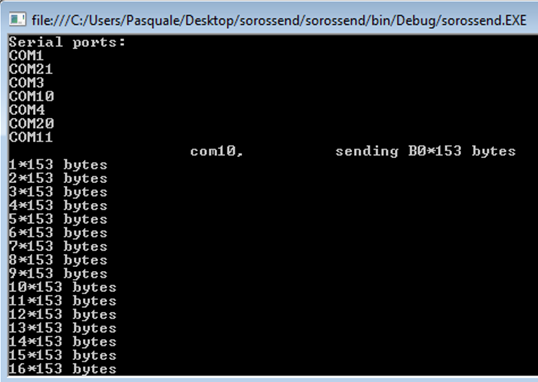
\includegraphics{figures/sorossend.png}}
	\caption{}
	\label{fig:sorossend}
\end{figure}

153 b�jtos egy csomag, melyet egy UUT  3 b�jtos fejl�c �s egy 2 b�jtos checksum z�r. A checksum a hasznos b�jtok 16 bitre csonkolt �sszege. Minden fogadott csomagn�l, a feldolgoz�s el�tt kisz�molom az �sszeget �s ellen�rz�m, az egyez�st, a rossz csomagok egyel�re eldob�sra ker�lnek.

\begin{figure}[!ht]
	\centering
	\resizebox{10cm}{!}{
		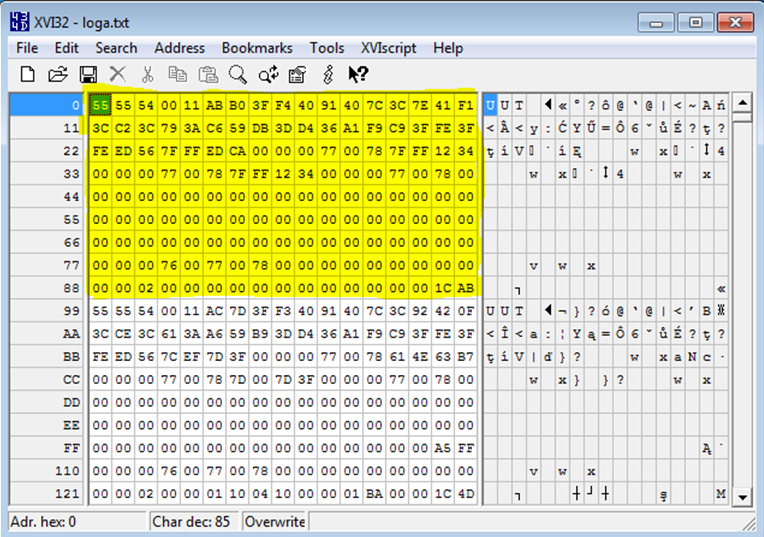
\includegraphics{figures/xvi.png}}
	\caption{}
	\label{fig:xvi}
\end{figure}

Fogad� oldalon a k�t sorosport aszinkron �r 1-1 byte t�mb�t, melyb�l egy dek�dol� f�ggv�nnyel nyerj�k ki a sebess�g, poz�ci�, ir�ny, stb. adatokat.

\begin{verbatim}
public double[] Decode(byte[] array)
\end{verbatim}

Ebben a f�ggv�nyben ellen�rz�m, a checksum-ot, illetve a kezd� UUT b�jt h�rmast.
Mivel b�jtos�val lehet feldolgozni az adatokat, �gy pl. a 4 b�jtos id�b�lyeget 4 db egym�s ut�n j�v� b�jtb�l kell �sszerakni:

\begin{verbatim}
uint ido = (uint)array[3]<<24 | (uint)array[4]<<16 |
(uint)array[5]<<8 | (uint)array[6];
\end{verbatim}

Ugyan�gy folytat�dik az adatok feldolgoz�sa, az el�re megadott protokoll szerint.

\begin{center}
    \begin{tabular}{| l | l | l | l |l |}
    \hline
    b�jt index & le�r�s & t�pus & sk�l�z�s & offset \\ \hline
    1 & start & char(fix 'U') &   &    \\ \hline
		2 & start & char(fix 'U') &   &    \\ \hline
		3 & start & char(fix 'T') &   &    \\ \hline
		4 & id� 1/4 & unsigned int & 10000 & 0  \\ \hline
		5 & id� 2/4 &   &   &    \\ \hline
		6 & id� 3/4 &   &   &    \\ \hline
		7 & id� 4/4 &   &   &    \\ \hline
		\dots &  &  &   &    \\ \hline
		26 & �szaki ir�ny 1/2 & unsigned short & 0x7FFF/400 &  200 \\ \hline
		28 & keleti ir�ny 1/2 & unsigned short & 0x7FFF/400 &  200 \\ \hline
		30 & lefel� ir�ny 1/2 & unsigned short & 0x7FFF/400 &  200 \\ \hline
		\dots &   &   &   &    \\ \hline
		
    \hline
    \end{tabular}
\end{center}


Mivel a v�ltoz�sok Hamming-t�vols�ga\footnote{Bin�ris sz�mok XOR k�pz�s�vel kapott 1-esek sz�ma} kicsi lenne, az eredeti sz�m�br�zol�son, �gy sk�l�z�ssal �s offset k�pz�ssel megn�velj�k. A sebess�g adatokn�l a visszak�dol�s:\\
$eredeti  = (nyers adat/skalazas) - offset$ k�plettel oldhat� meg. 

\section{Sebess�g}
A sebess�g NED\footnote{Nort East Down, Local Tangent Pane, helyi koordin�ta rendszer} koordin�tarendszerben van megadva, mely a rep�l� k�z�ppontj�b�l indul. Mivel kis magass�gban rep�l a rep�l�, �gy s�knak k�zel�thetj�k  a F�ld fel�let�t, ez sz�m�t�sok szempontj�b�l el�ny�s, mivel k�nnyebb vele dolgozni.
A sebess�g sz�m�t�si m�dja: $ \sqrt[2]{(V_E)^2 + (V_N)^2}$ \\
Emelked�s: $ -V_D$
\begin{figure}[!ht]
	\centering
	\resizebox{8cm}{!}{
		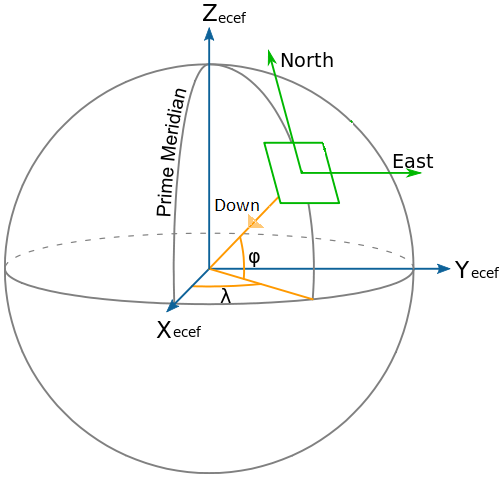
\includegraphics{figures/ned.png}}
	\caption{Koordin�ta rendszer}
	\label{fig:ned}
\end{figure}

\section{Ir�ny}
Az ir�ny meghat�roz�s�hoz a 4 negyeds�kot k�l�n kellett v�lasztani:
\begin{verbatim}
					if (Ecomp > 0 && Ncomp > 0)
					{
						heading = Math.Atan(Ecomp * Ncomp);
					}
					else if (Ecomp > 0 && Ncomp < 0)
					{
						heading = Math.Atan(Ecomp * Math.Abs(Ncomp)) + 90;
					}
					else if (Ecomp < 0 && Ncomp < 0)
					{
						heading = Math.Atan(Math.Abs(Ecomp) * Math.Abs(Ncomp)) + 180;
					}
					else if (Ecomp < 0 && Ncomp > 0)
					{
						heading = Math.Atan(Math.Abs(Ecomp) * Ncomp) + 270;
					}

\end{verbatim}

\section{GUI}
A grafikus fel�let kialak�t�sa sor�n figyelembe kell venni, hogy els� r�n�z�sre a legfontosabb adatok l�tsz�djanak. Kett� f�l k�z�l az els� oldalon a legfontosabb m�szerek tal�lhat�ak, jobb oldalon egy Google Maps t�rk�p. A t�rk�p egy lok�lis cache-b�l t�lti be az el�re let�lt�tt t�rk�pszelv�nyeket, �gy a terepen lehet\H{o}s�g van offline m�don is haszn�lni ezt a funkci�t.

%%----------------------------------------------------------------------------
\chapter{�rt�kel�s}
%----------------------------------------------------------------------------

\textbf{Megtervezett m�szaki alkot�s �rt�kel�se, kritikai elemz�se, tov�bbfejlesztet�si lehet�s�gek}
\chapter{�sszefoglal�s}\label{sect:}

SZUMM
%%----------------------------------------------------------------------------
\chapter*{K�sz�netnyilv�n�t�s}\addcontentsline{toc}{chapter}{K�sz�netnyilv�n�t�s}
%----------------------------------------------------------------------------

Ez nem k�telez�, ak�r t�r�lhet� is. Ha a szerz� sz�ks�g�t �rzi, itt lehet k�sz�netet nyilv�n�tani azoknak, akik hozz�j�rultak munk�jukkal ahhoz, hogy a hallgat� a szakdolgozatban vagy diplomamunk�ban le�rt feladatokat sikeresen elv�gezze. A konzulensnek val� k�sz�netnyilv�n�t�s sem k�telez�, a konzulensnek hivatalosan is dolga, hogy a hallgat�t konzult�lja.

%\listoffigures\addcontentsline{toc}{chapter}{�br�k jegyz�ke}
%\listoftables\addcontentsline{toc}{chapter}{T�bl�zatok jegyz�ke}

%\bibliography{mybib}
%\addcontentsline{toc}{chapter}{Irodalomjegyz�k}
%\bibliographystyle{plain}


\begin{thebibliography}{9}


\bibitem{bib:uav}
http://www.azom.com/article.aspx?ArticleID=10156, 2013.~november~19, 10:00

\bibitem{bib:canwiki}
http://hu.wikipedia.org/wiki/CAN\_bus, 2013.~december~12., 11:00

\bibitem{bib:xbee}
http://www.digi.com/products/wireless-wired-embedded-solutions/zigbee-rf-modules/point-multipoint-rfmodules/xbee-pro-868, 2013.~okt�ber~29, 14:00

\bibitem{bib:startxbee}
http://www.makershed.com/v/vspfiles/assets/images/122-32450-xbeetutorial-v1.0.1.pdf, 2013.~december~12., 11:00

\bibitem{bib:ieee}
http://standards.ieee.org/getieee802/download/802.15.4-2011.pdf, 2013.~november~29, 15:00

\bibitem{bib:zigbee}
http://www.digi.com/pdf/wp\_zigbee.pdf, 2013.~november~29, 14:00

\bibitem{bib:osiwiki}
http://hu.wikipedia.org/wiki/OSI\_modell, 2013.~december~12., 11:00

\bibitem{bib:network}
http://www.sensor-networks.org/?page=0823123150, 2013.~december~02, 22:00

\bibitem{bib:aimofuav}
http://www.uvisionuav.com/portfolio/gcs/, 2013.~november~24., 15:00

\bibitem{bib:multimodal}
http://personal.us.es/imaza/papers/journals/maza\_jint10\_multimodal/maza\_jint10\_multimodal\_web.pdf, 2013.~november~24., 15:00

\bibitem{bib:ardu}
https://code.google.com/p/ardupilot-mega/wiki/Mission, 2013.~november~24., 15:00

\bibitem{bib:arduino}
http://arduino.cc/, 2013.~december~11., 23:00

\bibitem{bib:paparazzi}
http://paparazzi.enac.fr, 2013.~november~24., 15:00

\bibitem{bib:micropilot}
http://www.micropilot.com/products-horizonmp.htm, 2013.~november~24., 15:00

\bibitem{bib:makkay}
http://www.szrfk.hu/rtk/kulonszamok/2012\_cikkek/77\_Makkay\_Imre-Papp\_Timea.pdf, 2013.~november~24., 15:00

\bibitem{bib:openpilot}
http://wiki.openpilot.org/display/Doc/OpenPilot+Documentation, 2013.~november~24., 15:00

\bibitem{bib:qground}
http://qgroundcontrol.org/, 2013.~november~25., 15:00

\bibitem{bib:hk}
https://code.google.com/p/ardupilot-mega/wiki/HappyKillmore, 2013.~m�rcius~19., 16:00

\bibitem{bib:serial}
http://msdn.microsoft.com/en-us/library/system.io.ports.serialport.aspx, 2013.~m�rcius~20, 10:00

\bibitem{bib:netstart}
http://msdn.microsoft.com/en-us/library/hh425099.aspx, 2013.~december~5, 12:00

\bibitem{bib:net}
http://msdn.microsoft.com/en-us/library/zw4w595w.aspx, 2013.~december~5, 12:00

\bibitem{bib:aut}
https://www.aut.bme.hu/Course/VIAUA218, 2013.~december~5, 12:00

\bibitem{bib:gdi}
http://msdn.microsoft.com/en-us/library/windows/desktop/ms533798.aspx, 2013.~december~3, 12:00

\bibitem{bib:gmap}
http://greatmaps.codeplex.com/, 2013.~december~8, 11:00

\bibitem{bib:null}
http://com0com.sourceforge.net/, 2013.~m�jus~4, 10:00


\end{thebibliography}

%----------------------------------------------------------------------------
\appendix
%----------------------------------------------------------------------------
\chapter*{F�ggel�k}\addcontentsline{toc}{chapter}{F�ggel�k}
\setcounter{chapter}{6}  % a fofejezet-szamlalo az angol ABC 6. betuje (F) lesz
\setcounter{equation}{0} % a fofejezet-szamlalo az angol ABC 6. betuje (F) lesz
\numberwithin{equation}{section}
\numberwithin{figure}{section}
\numberwithin{lstlisting}{section}
%\numberwithin{tabular}{section}

%----------------------------------------------------------------------------
\section{Program elind�t�sa}
%----------------------------------------------------------------------------

Ahhoz, hogy a programot �rdemlegesen lehessen futtatni, a \sectref{fejlesztes} fejezetben ismertetett programok telep�t�s�t �rom le.

A program futtat�s�hoz Windows XP/Vista/7 �s .NET 4.5-s verzi� sz�ks�ges. A .NET keretrendszer telep�t�je a mell�kleten \textit{dotNetFx45.exe}\footnote{Internet el�r�s sz�ks�ges} n�ven szerepel. 

A rep�l�g�ppel t�rt�n� kommunik�ci� szimul�l�s�hoz sz�ks�ges egy nullmodem telep�t�se. A telep�t�st k�vet�en l�tre kell hozni a COM10-COMXX �s COM20-COMYY p�rokat. Windows7 x64 rendszeren a \textit{com0comW7.exe} telep�t�se, m�g XP eset�n a \textit{com0comXP.zip} telep�t�se aj�nlott. A COM10 �s COM20 portokat fixen a log file beolvas�s�t v�gz� konzolos programok haszn�lj�k, az XX-szel �s YY-nal jel�lt portok szabadon v�laszthat�k.

Ha k�sz az �sszek�ttet�s, akkor a \textit{sorossendA.exe} �s \textit{sorossendB.exe} futtat�s�val a log f�jlok a soros portokra �r�dnak. A \textit{GroundControl.exe} program ezek ut�n ind�that�, a portok kiv�laszt�s�t k�vet�en l�that� a t�nyleges m�k�d�se. A kapott log f�jlok San Francisco repter�n k�sz�ltek HIL (Hardware In the Loop)\footnote{olyan szimul�ci�, ami a tesztelend� be�gyazott rendszernek olyan k�rnyezetet biztos�t, mintha az val�di �rz�kel�k adatait fogadn� �s val�di aktu�torokat ir�ny�tana} szimul�ci�val.



%----------------------------------------------------------------------------
\section{T�rk�p let�lt�se}
%----------------------------------------------------------------------------
\label{sect:gmap}

�j ter�let let�lt�s�re a mell�klet \textit{GMap.Net/Demo.WindowsForms.exe} programja haszn�land�. A program t�rk�pes fel�let�n �j ter�letet Alt billenty� hosszan nyom�s�val �s eg�r mozgat�s�val lehet kijel�lni. Ezt k�vet�en, a ``cache'' f�l�n a ``Prefech'' gomb hat�s�ra kiv�laszthat� r�szletezetts�ggel let�lt�dik. Az ``Export'' gombra kattintva a let�lt�s hely��l a \textit{/map/TileDBv5/en/} �tvonalon tal�lhat� \textit{Data.gmdb} f�jlt kiv�lasztva fel�l�rhat� az offline t�rk�pszelv�ny.

\begin{figure}[H]
	\centering
	\resizebox{8cm}{!}{
		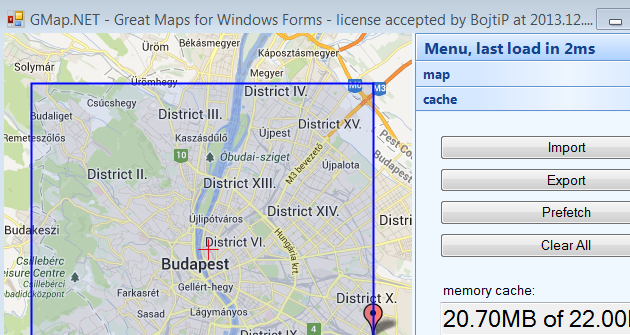
\includegraphics{figures/gmap.png}}
	\caption{}
	\label{fig:gmap}
\end{figure}

\label{page:last}

\end{document}
